\documentclass[a4paper,oneside]{report}

\usepackage{amsmath}
\usepackage{amssymb}
\usepackage{caption}
\usepackage[english]{babel}
\usepackage{fancyhdr} 
\usepackage{float}
\usepackage{multirow}
\usepackage[pdftex]{graphicx}
\usepackage{listings}      
\usepackage{pdfpages}
\usepackage{setspace}
\usepackage{url}
\usepackage{wrapfig}

\lstset{language=C,
numberstyle=\footnotesize,
%basicstyle=\ttfamily\footnotesize,
basicstyle=\footnotesize,
numbers=left,
stepnumber=1,
frame= lines,
breaklines=true}

\makeatletter


%
% Some custom definitions
%

% add horizontal lines
\newcommand{\HRule}{\rule{\linewidth}{0.5mm}}
\newcommand{\HRuleLight}{\rule{\linewidth}{0.1mm}}

% custom part page
\def\part#1#2
{
	\par\break
  	\addcontentsline{toc}{part}{#1}
	\noindent
	\null	
	\HRuleLight\\[0.0cm]
	\vspace{20pt}	 
	\begin{flushright} 		
  	{\Huge \bfseries \noindent #1}\\
  	\vspace{30pt} 
	\begin{minipage}{0.85\textwidth}
		\begin{flushright}
		{\large \noindent #2}
		\end{flushright}
	\end{minipage}\\[0.75cm] 
	\end{flushright} 		
	\thispagestyle{empty}
	\break
}

% chapter header
\renewcommand{\@makechapterhead}[1]
{\vspace*{50\p@}{
	\parindent \z@ \raggedright \normalfont
	%\huge \bfseries \thechapter. #1
	\huge \bfseries #1
	\vspace{20pt}}}

\setcounter{secnumdepth}{-1} 
\onehalfspace
\oddsidemargin 1in 
\oddsidemargin 0.6in 
\topmargin -0.3in
\setlength{\textwidth}{14cm}
\setlength{\textheight}{23cm}
\lstset{language=C} 

\begin{document}

%
% Cover page
%
\begin{titlepage}
\begin{center}


\includegraphics[width=120mm]{sources/images/cogito_logo_main.png}

\HRuleLight\\[0.5cm]

\begin{minipage}{0.45\textwidth}
	\begin{flushleft}\large
		\emph{Author:}\\
			\textbf{Thomas \textsc{Taylor}}\\[0.27cm]
			Computer Science (Games)
			Student Number: 08813043
	\end{flushleft}
\end{minipage}
\begin{minipage}{0.43\textwidth}
	\begin{flushright} \large
		\emph{Supervisor:} \\
		\textbf{Graham \textsc{Winstanley}}\\[0.25cm]
		\emph{Second Reader:}\\
		\textbf{Saeed \textsc{Malekshahi}}
	\end{flushright}
\end{minipage}\\[0.75cm] 

\HRuleLight\\[0.2cm]

\large School of Computing, Engineering and Mathematics\\ \textbf{University of Brighton}

\vfill
\huge Project Documentation\\
\large April, 2012\\

\end{center}
\end{titlepage}



%
% Table of contents
%
{
	\renewcommand\thepage{}
	\setcounter{tocdepth}{1}
	\tableofcontents
	\clearpage
}

% reset page count
\setcounter{page}{1}


%
% Start of content
%

\chapter{Introduction}

The artificial intelligence (AI) techniques used by game developers today are archaic in comparison to the techniques used by academic AI researchers. Indeed, the A* search algorithm is still one of the most popular AI algorithms used in games today, and was first introduced in academic AI over 30 years ago. That being said, it is important to view such techniques in the context of which they are used: while academic AI researchers are free to use as much processing power as the hardware can afford them, game developers are much more limited, as said resources must be shared with many other processes such as physics, sound, networking and graphics. For this reason, it is understandable that game developers want to squeeze as much functionality as possible from the least amount of processor time. The fact is that modern game AI programming is more a skill of giving the illusion of intelligence than actually providing it. This means that shortcuts and workarounds are a common necessity in order to achieve `believable' AI with the resources available. 

That being said, we are starting to see a change taking place in the computer game industry which suggests that AI is being taken more seriously, and given much higher priority than it has in the past. One factor in this change is the so-called `graphics plateau': it has been said that we have now reached an `acceptable' level of graphical complexity such that we are unlikely to see any more major advances in the field \cite{Sheffield:2008fk}. This being true, and given the current rate of hardware advancement, we are sure to see much more processor time freed up for those processes such as AI which have been treated as `extraneous' in the past. Another important factor in this change is the emergence of the `casual' gamer. With casual games now accounting for a considerable proportion game sales, the consumer has shown that there is a big market for games which have less emphasis on complex graphics effects, and more emphasis on interesting gameplay mechanics \cite{Association:2011uq}. Indeed, with Nintendo's Wii home console having far outsold both Sony's PlayStation 3 and Microsoft's Xbox, the consumer has shown that they value unique gameplay and accessibility over advanced graphics \cite{:2012dq, Nintendo:2012nx, :cr}. 

With these factors already starting to bring about a change in the priority that developers give to the components of their games, I believe that now is as good a time as any for developers to introduce some more advanced AI techniques into their games.

\section{Project Aims and Objectives}

The main aim of my project was to experiment with some more advanced academic AI techniques which are not typically found in commercial games, and look into whether such techniques were viable with today's hardware. This second point is key, especially given the popularity of `limited' hardware such as the Nintendo Wii, and mobile devices.

The sub-field of AI that I chose to focus my project on was machine learning, as it is an emerging field which greatly interests me and one which I feel is a natural fit for computer games, and one we could see utilised in many forms in future games.

For my project, I wanted to develop an AI system which was capable of employing machine learning techniques in order for a number of AI-controlled agents to safely navigate a 2D game environment. I wanted the agents to be able to develop a knowledgebase dynamically, with no need for prior training, or knowledge of the game world. I then wanted the agents to be able to apply this gained knowledge in order to hopefully increase their chances of survival. 

\section{Background}

I chose the classic Commodore Amiga game `Lemmings' as the context and main inspiration for my project.

\begin{wrapfigure}{r}{0.61\textwidth}
  \centering
    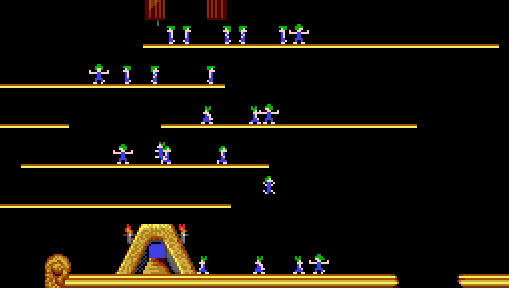
\includegraphics[width=80mm]{sources/images/lemmings3}
    \caption{A typical level in Lemmings.\label{screen}}
\end{wrapfigure}

Originally released in 1991 for the PC and Commodore Amiga, `Lemmings' has a very simple premise: to guide a group of computer-controlled `Lemmings' across a level from the entrance-point to the exit. The Lemming characters themselves have no real AI to speak of, and are capable of merely walking across the level. The level itself consists of a number of platforms which the Lemmings must navigate whilst avoiding various hazards (such as big drops, pits etc.). To aid in this task, the player is given a number of tools such as umbrellas for big drops and girders to cross pits. Interestingly, a student at Rutgers University has shown that this is actually an NP-Hard problem \cite{Cormode:fk}.

For my project, I planned to take this concept, simplify it by removing some of the tools and obstacles, and program some AI agents to learn for themselves how to best traverse the level, without any human interaction.



%
% New part
%

\part{Research}{This section documents the research that I carried out prior to designing my system, and how it influenced my final designs. \\ \ \\The section is split into two subsections: my research into AI, and my research into the more game-related topics.}

\chapter{Artificial Intelligence}

Since the early days of computing, computer scientists have striven to replicate in machines the defining characteristic that makes us human: intelligence. One of the first references to `intelligent machines' came in 1950 in Alan Turing's seminal paper \emph{Computing Machinery and Intelligence}, in which Turing opens with the words: "I propose to consider the question, 'Can machines think?'". In it, he outlines a test in which a human participant engages in conversation with a machine designed to imitate human behaviour, known as the Turing Test. This paper also inspired us to look philosophically at what it is that makes us inherently human, and whether this is indeed replicable in a machine.

The term `artificial intelligence' was later formally defined in 1955 by McCarthy et al in the proposal for the Dartmouth Summer Research Conference on Artificial Intelligence, which is considered by many to be the origin of the field of AI \cite{Crevier:1993kl}. In the proposal, it was suggested that ``every aspect of learning or any other feature of intelligence can in principle be so precisely described that a machine can be made to simulate it" \cite{McCarthy:1955ve}. Since these early days, the field of AI has grown to become an integral field not only in computer science, but also in the infrastructure of every industry \cite{Kurzweil:2005ly}. 

\section{AI In Games}

One area where AI techniques are used extensively is computer games. Whether to map a route across obstacle-ridden terrain, control the actions of non-player characters (NPCs) or even to adjust game parameters to fit to the skill of the player, AI plays a key role in almost all modern computer games. However, due to the nature of the final product, game AI takes a very contrasting approach to that of academic AI. While the aim with academic systems is always to provide the most complete and accurate results, the ultimate aim with game AI is to provide entertainment for the user by giving the illusion of intelligence. Ironically, this can often mean that it is necessary to make the system intentionally `stupid' by building flaws in the system or even by allowing the system to cheat to ensure that the game AI behaves `realistically' \cite{Liden:2004fk}. Additionally, academic AI systems usually have very simplistic visualisation, allowing the majority of processing time to be dedicated to the AI. Game AI on the other hand, must run simultaneously with a number of other processes such as the physics engine, sound and most significantly graphics which in reality means that the AI processing is often compromised in the favour of other processes. In the proceeding sections, I outline some of the most popular AI techniques used in commercial computer games today.

\subsection{Finite State Machines} 

Finite state machines (FSMs) are one of the most commonly used AI techniques found in games today. As the name suggests, FSMs are ``simple, rule-based systems in which a finite number of 'states' are connected in a directed graph by 'transitions' between states" \cite{:hc}. One of the first games to sucessfully use FSMs was Atari's 1979 game \emph{Pacman}, in which the enemy ghost characters use a FSM to define states (chase, run away and roam), changing their state in response to in-game triggers. FSMs are used extensively in many commercial games, as they are relatively easy to understand, implement and debug \cite{Bourg:2004tg}.

\subsection{Search and Planning Systems} 

Search systems are primarily concerned with finding actions/states in a graph to satisfy a goal condition (or at least to get as close as possible). Planning systems are a specific branch of search which have an emphasis on finding the best (or simplest) sequence of actions required in order to reach the goal state. Many algorithms have been developed, but the A* algorithm is the one used most extensively, due to its performance and the accuracy of its results. Search and planning systems are used for a variety of tasks, from the pathfinding of AI agents in a first-person shooter game to the allocation of resources in a real-time strategy game. Blizzard's 1994 game \emph{Warcraft} is an example of an early implementation of using the A* pathfinding algorithm to navigate agents.

\subsection{Artificial Life} 

An artificial life (A-life) system is designed to exhibit realistic and lifelike behaviour in game characters. A-life systems are often used to coordinate the movement of multi-agent systems to make the agents manoeuvre in flock and herd formation. One of the most compelling reasons to use A-life techniques is that more complex behaviours can emerge from the pre-programmed rules \cite{Woodcock:bs}. \emph{The Sims} developed by Maxis (now part of EA) is probably one of the best known games to use A-life techniques, and uses so-called `smart terrain' to broadcast information to the game characters. For example, a hungry character may walk past a refrigerator, which broadcasts that it contains food. After collecting the food, the nearby oven broadcasts that it can cook the food, leading the character to it \cite{Woodcock:bs}. These individual object-level actions when combined, cause the character to exhibit realistic `emergent' behaviour which, while very useful, is also incredibly difficult to debug. Additionally, the techniques can be incredibly processor intensive, making them unsuitable for some games. 

\subsection{Scripting} 

Another popular technique in game AI is scripting, whereby developers use a specialised high-level scripting language to outline the NPCs reactions to basic situations and hard-code game events. Scripting allows the game engine to be accessed externally in a safe `sandbox' environment, greatly reducing the chance of bugs and errors, so is suitable for non-programmers such as designers. For this reason, there is a large community of gamers who use scripting interfaces to create additional game content. Lionhead Studios used scripting heavily in their 2001 game \emph{Black \& White} to present the game's storyline using a series of in-game challenges rather than more traditional cut-scenes \cite{:hc}. A big disadvantage to using scripting is that it requires every character behaviour and game scenario to be hard-coded which is incredibly time consuming for the programmer/developer, and is not always possible. Additionally, using scripting can be very restrictive for the player, as the story progression is often very linear.

\subsection{Cheating The System}

Game developers also use a number of hacks and workarounds to give their AI systems the illusion of intelligence while retaining the entertainment value; in many cases, traditional AI techniques are unnecessary. In computer games, entertainment is paramount, and so it may be inappropriate to implement a very `smart' adaptive AI system. Consider Konami's stealth-action series \emph{Metal Gear Solid} in which the player must navigate a level while avoiding detection from the guard NPCs. Using a truly intelligent and adaptive AI system would remove a lot of the entertainment value of the game which in which the player must recognise patterns in guard behaviour in order to progress. While this AI system would be considered flawed in the eyes of an academic researcher, it is perfectly acceptable (even preferable) in the context of the game. Game developers also afford the AI system extra information or resources unavailable to the player. This is particularly useful in real-time strategy games to give the computer access to extra troops or supplies. Using these kinds of `cheats' can be an acceptable way to increase the level of difficulty, although it can be a challenge to disguise this from the player; if the player feels that the game is acting unfairly and that their actions are ineffective, they will obviously not enjoy the game.

\subsection{The Future of Game AI}

From as early as 2000, statistics were showing that the industry was beginning to take AI more seriously. Figures collected from the AI roundtable at the annual Game Developer's Conference showed that not only were a lot more studios employing dedicated AI programmers, but that the average amount of CPU time reserved for AI processing increased from 5\% to over 25\% \cite{Woodcock:oq}.

\section{Machine Learning}

\begin{quotation}``A computer is said to learn from experience \emph{E} with respect to some class of tasks \emph{T} and performance measure \emph{P}, if its performance at tasks in \emph{T}, as measured by \emph{P}, improves with experience \emph{E}." - \textbf{Tom Mitchell} \cite{mitchell1997machine} 
\end{quotation}

The ability to learn is one of the central features of intelligence \cite{Langley:1996zr}. To then apply this knowledge and modify behaviour accordingly when faced with similar scenarios is an area which has received a considerable amount of research. In fact, machine learning techniques are already in use in a number of commercial applications such as speech recognition, robotic control and machine vision, proving that it can be a very useful solution, especially in solving problems which may have unexpected outcomes that cannot be predicted by the software developer.

\paragraph{Online and Offline:} Learning which takes place while a system is running is said to be `online', while `offline' learning refers to a system which modifies its behaviour \emph{after} it has finished running. Whilst online learning provides instantaneous results, it also makes the system much more difficult to debug were any issues found, due to its continuous modification.

\paragraph{Supervised and Unsupervised:} Learning which utilises example training data is described as `supervised', whereas a system which only has access to the data that it collects itself is described as `unsupervised'. The benefit to supervised learning is that the system can base its learning on some correct `solutions', which leads to more accurate and perhaps `quicker' learning. However, the training data itself needs to be collected and analysed, which requires human input, and can become very time consuming. Unsupervised methods on the other hand do not have this requirement, but must analyse the collected data to find hidden structure; there is no `correctness' indicator to evaluate potential solutions. There are also techniques which form an intermediary between the two, using both labelled and unlabelled data. These methods are known as `semi-supervised'.

\subsection{Reinforcement Learning}

Reinforcement learning (RL) is the name given to the subset of machine learning techniques which use a reward system to let the system know how it is performing. The overall aim of RL being to maximise the cumulative reward. RL uses a cause and effect loop whereby the system begins in a state, performs an action (receiving a reward), which causes the environment to change its state, repeating the cycle (see Figure \ref{fig:Screen}).

\begin{wrapfigure}{r}{0.5\textwidth}
  \centering
    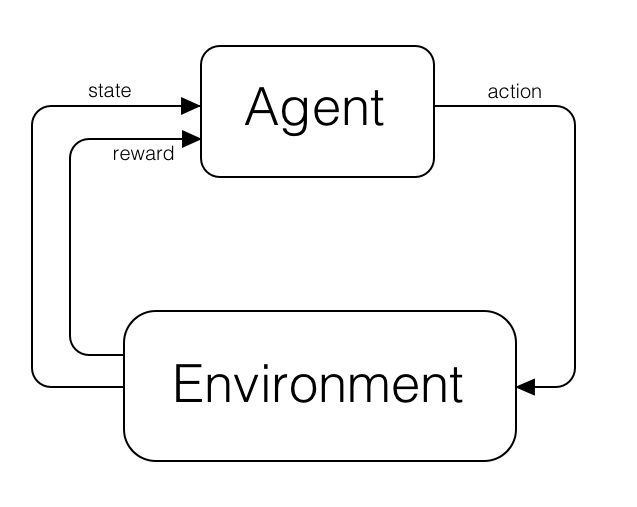
\includegraphics[width=70mm]{sources/images/RLDiagram}
    \caption{Reinforcement Learning Loop \cite{Nilsson:2010qa}.}
    \label{fig:Screen}
\end{wrapfigure}

What sets RL apart from other types (supervised/unsupervised methods) is that the learner is never given correct input/output, nor are any incorrect actions ever corrected, leaving the system to deduce where an error has occurred. This can be particularly tricky to ascertain as an error can often occur due to a poor decision made several time-steps in the past. Similarly, the mistake could have been made as a result of 20 previous actions, all of which would have to be repeated in sequence to replicate the error. This is known as the `credit assignment problem', and results from the fact that RL uses a sequential style of learning, where a system makes many decisions which lead to an eventual goal condition. In an attempt to combat this, RL introduces the notion of `regret', by taking into account the long-term effects of actions. As a result of this, an RL system may choose an action with a negative immediate reward so as to maximise its long-term reward. RL also involves finding an acceptable compromise between exploration (of new undiscovered terrain) and exploitation (of the system's current knowledgebase).

RL algorithms are split into two main categories: dynamic-programming-based (which themselves are not strictly RL), and the `truly' RL algorithms. Which algorithms can be used depends on the information we have about the environment. If the state transition probabilities and the reward functions for the environment are already known, we can calculate the optimal policies using standard dynamic-programming techniques such as value-iteration and policy-iteration. First described by Richard Bellman, dynamic programming aims to solve problems by simplifying them into subproblems and solving those recursively. If on the other hand, we do not know state transition probabilities, the policy must be learned using `true' RL algorithms such as Q-learning.

\subsubsection{Markov Decision Processes:}

Markov decision processes (MDPs) are often used to model the environment in which the system is intended to be used. An MDP is usually represented as: $MDP(S, A, \{Psa\}, \gamma, R)$ and consists of 5 main components: 

\begin{enumerate}
	\item A set of possible states \emph{S}
	\item A set of available actions \emph{A}
	\item Probability \emph{P} of moving from the current state \emph{s} to a new state \emph{$s^\prime$} by taking action \emph{a}
	\item The discount factor $\gamma$ where 0 $\leq \gamma \leq$ 1 (adjusts the influence of future rewards)
	\item A reward function \emph{R}, which maps from a state to a real number $R : S \mapsto \mathbb{R}$ 
\end{enumerate}

\subsubsection{The Theory} 

In order for the algorithms to compute an optimum policy, the system must first build up a knowledgebase through experience. It does this simply by executing:

\begin{enumerate}
	\item Starting in state $s_0$, it performs action $a_0$ (often chosen at random during this learning phase), causing the system to move to a new state $s_1$ according to the probability function for $s_0$ and $a_0$ (e.g. a robot may have an inaccurate direction sensor, which when set to move north, causes it to move north 80\% of the time, with a 10\% of going east, and a 10\% chance of going west).
	\item After running for an amount of time, the system will have reached a number of states ($s_0, s_1, s_2, s_3 ...$) The performance of the system can then be evaluated using a reward function, whereby the cumulative rewards would be: \\
	$R(s_0) + R(s_1) + R(s_2) + R(s_3) + ...$
	\item The final step is to factor in a discount factor, which gives us: \\
	$R(s_0) + \gamma R(s_1) + \gamma^2 R(s_2) + \gamma^3 R(s_3) + ...$ \\ (Whereby the reward received at time-step $t$ is discounted by $\gamma^t$, which gives a greater weighting to rewards now than to rewards in the future).
\end{enumerate}

The ultimate goal of the RL algorithm is to formulate a policy\footnote{The term `policy' is used to refer to a set of action/state mappings often symbolised by $\pi$} $\pi$ which maps states to actions ($\pi: S \mapsto A$) such that for every state, the policy recommends the optimum action to take. After a certain number of iterations of the algorithm, the policy's values become static (i.e. they are no longer updated). This signifies that the optimum policy has been found, and the values have \emph{converged}. This could take as little as a few thousand iterations for small problems, but more likely will take many more. In many real-world cases, there may not be enough time to reach convergence, in which case the best policy would be used.

\subsubsection{Algorithms}

There have been a variety of different RL algorithms developed, each with their own advantages and disadvantages. Some examples are Temporal Difference, Monte Carlo, Bucket Brigade and Q-learning which is described in more detail below.

\subsubsection{Q-learning}

Originally proposed by Christopher Watkins in 1989 \cite{Watkins:1989mi}, Q-learning takes a slightly different approach to other RL algorithms, as it doesn't require a complete model of the environment, which can be a big advantage as it is not often not possible (or indeed feasible) to generate a model before the system has run. Q-learning gets its name from the quality information, or Q-values which it stores for each possible action in every state of the system. This Q-value represents how `good' the system thinks that an action is to take when in a given state.

\noindent The Q-learning algorithm is as follows:
\begin{equation*}
	Q(s_t,a_t) \Leftarrow Q(s_t, a_t) + \alpha_t(s_t, a_t)[R(s_t) + \gamma max_{a_{t+1}} Q(s_{t+1}, a_{t+1}) - Q(s_t, a_t)]
\end{equation*}

\noindent But is often rewritten more simply as:
\begin{equation*}
	Q(s_t,a_t) \Leftarrow Q(s_t, a_t) + (1 -\alpha_t) + \alpha[R(s_t) + \gamma max Q(s_{t+1}, a_{t+1})]
\end{equation*}

Where $Q(s_t, a_t)$ represents the Q-value for the current state/action, $R(s_t)$ represents the reward associated with the current state and $max Q(s_{t+1}, a_{t+1})$ represents the maximum possible Q-value for the next state. Q-learning also introduces and addition variable known as the learning rate (represented as $\alpha$), which affects how quickly the Q-values are modified; a greater learning rate results in much faster changes to Q-values. It is common practice to begin with a large learning rate, and decrease it as time goes on, to fine-tune the Q-values. Researchers at Tel-Aviv University carried out some interesting research into the effect of learning rates on the rate of convergence, which suggests that convergence can be reached much quicker if using a variable learning rate \cite{Even-Dar:2003jl}.

Updating the old Q-values ensures that the system retains all previously obtained knowledge. Introducing the max Q-value into the equation means that the success (or failure) of an action is reflected in earlier actions, in effect `trickling' back up the supply chain.

Q-learning converges with probability 1, meaning that after sufficient iterations of the algorithm, the learner will have formulated an optimal policy such that they can move towards the most desirable state from any other state.

\subsection{Decision Trees}

Another popular type of machine learning is Decision Tree Learning. Decision Tree Learning approaches problem solving using classification to label input data. A tree structure is used to do this, with each node of the tree representing a test. The leaf nodes usually represent categories, although they can also represent numerical values. Each of these tests serve the function of sorting (or refining) the input data, with each possible answer being mutually exclusive (i.e only one answer can be satisfiable per test). The tests can be multivariate, where multiple attributes are tested at once, or univariate where only a single attribute is tested. As the input data moves down the tree, it will eventually filter through to a leaf (or category) node. See Figure \ref{fig:DecisionTree} for an example decision tree.

\begin{figure}[h!]
	\centering
		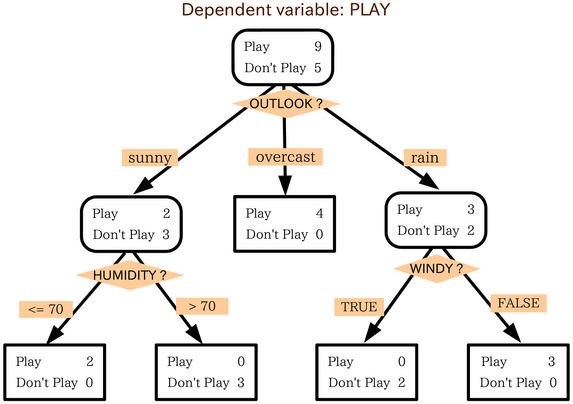
\includegraphics[width=100mm]{sources/images/DecisionTree}
    	\caption{An Example Decision Tree \cite{Koboldt:kx}}
    	\label{fig:DecisionTree}
\end{figure}

When building a decision tree, the ultimate goal is to order the tests in the tree in such a way that each level gives the maximum reduction in the entropy (or uncertainty). This is known as uncertainty reduction. There have been various algorithms developed to construct decision trees, the majority of which use a top-down approach. Among these are the ID3 and C4.5 algorithms (both developed by Ross Quinlan), and CART (developed by Leo Breiman et al) \cite{Quinlan86inductionof,Quinlan:1993:CPM:152181,breiman1984classification}.

One of the main benefits to using decision trees is that they are relatively easy to visualise and understand. Another key advantage is that tree structures are very commonly used in computer science, and so there exist various highly optimised algorithms for the building and searching of trees.

However, decision trees can lack accuracy; the size of the tree will increase tremendously if a much higher resolution output is required \cite{schwab2004ai}. Additionally, decisions trees do not scale well, with very large, highly complex trees being very difficult to maintain. Another important point to mention is that because game AI systems are required to learn online as the game is played, supervised techniques such as back propagation are inappropriate. Another issue related to decision trees is that of replicated subtrees, where certain portions of a tree are repeated (see Figure \ref{fig:ReplicatedSubtrees}).

\begin{figure}[h!]
	\centering
		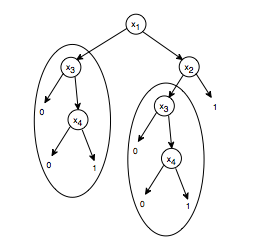
\includegraphics[width=60mm]{sources/images/ReplicatedSubtrees}
    	\caption{Replicated Subtrees}
    	\label{fig:ReplicatedSubtrees}
\end{figure}

\subsection{Genetic Algorithms}

Genetic algorithms are possibly one of the most interesting machine learning techniques. Taking inspiration from the process of natural evolution, they use a selection-reproduction-mutation process to create systems which are capable of not only determining the optimum behaviour from pre-programmed behaviour, but are also able to develop new emergent behaviour by cross-breeding and mutating existing behaviour. As with natural evolution, the process begins with an initial population of `chromosomes'. This initial population is often initialised randomly, but can be initialised to any arbitrary values desired by the programmer. After initialisation, the process uses a `generational' approach:

\begin{enumerate}
	\item Each chromosome in the population is evaluated using a `fitness' function which evaluates its effectiveness.
	\item From this, the system identifies the `fittest' chromosomes, and selects them to breed a new generation of chromosomes.
	\item The system then `breeds' the selected individuals. This process involves combining two `parent' chromosomes to create a child with a mixture of behaviour from both parents. See Figure \ref{fig:Breeding} for a graphical representation of this process.
	\item \emph{Many systems also introduce a `mutation' function which randomly selects individuals from the population and slightly alters them. This encourages emergent behaviour.}
	\item The resulting chromosomes form the new `generation' of behaviour to be used in the next iteration of the algorithm. This process is then repeated an arbitrary number of times until a certain number of iterations has been reached, or until a certain level of fitness has been achieved (as specified by the fitness function).
\end{enumerate}
  
\begin{wrapfigure}{l}{0.32\textwidth}
	\centering
		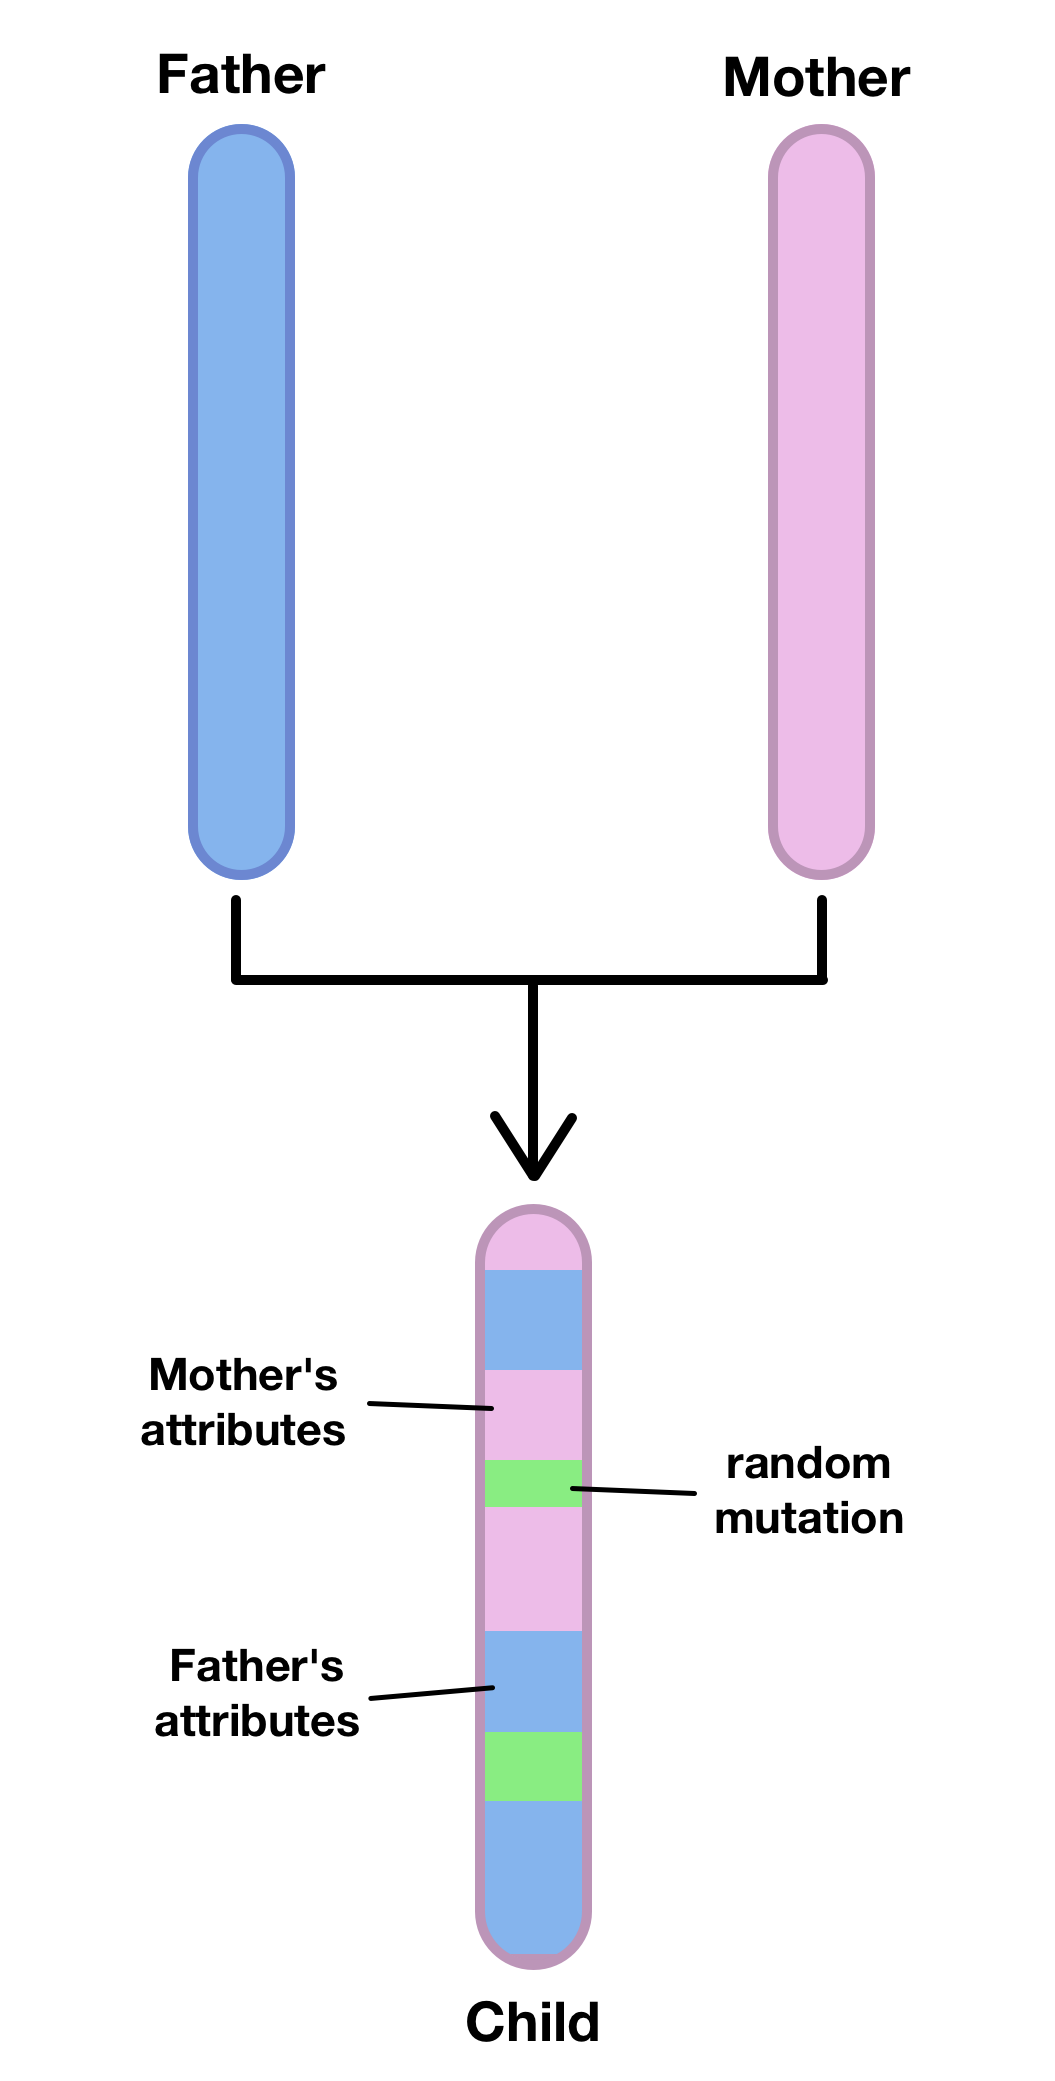
\includegraphics[width=50mm]{sources/images/Evolution}
    	\caption{The Breeding/Mutation Process}
    	\label{fig:Breeding}
\end{wrapfigure}

One of the biggest advantages to using genetic algorithms is that they encourage emergent behaviour through the breeding/mutation process. This is a big benefit to the programmer as they can be used in problems which don't necessarily have a clear solution. They are also fairly inexpensive computationally, so are well-suited to situations where it may be infeasible to explicitly calculate a decision. Genetic algorithms are often used to complement other AI techniques.

However, this being said, there are also a few disadvantages to using genetic algorithms. One such problem being that the actual evolution process can be very time consuming; it is likely to take many generations for a solution to be found. Additionally, depending on what the end condition for the algorithm is, it may be that no optimum solution is found (if the algorithm is set to run for a finite number of generations rather than ending when the population is deemed satisfactory by a fitness function). One final point to note is that genetic algorithms aren't well suited to systems which don't have a fixed design; if additional features are added, it can mean that the genetic algorithm may need to be completely redesigned.

\subsection{Artificial Neural networks}

\begin{wrapfigure}{r}{0.55\textwidth}
	\centering
		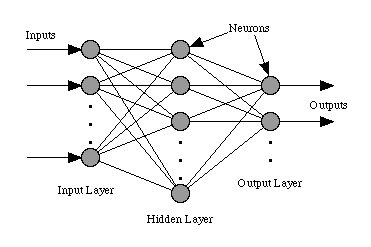
\includegraphics[width=80mm]{sources/images/NeuralNetwork}
    	\caption{An Artificial Neural Network \cite{Dawson:2000uq}}
    	\label{fig:NeuralNet}
\end{wrapfigure}

Artificial Neural Networks (NNs) are another popular machine learning technique which are inspired by the parallel architecture of the brain. NNs consist of a group of processing nodes (or neurons) which are interconnected in a graph structure (see Figure \ref{fig:NeuralNet} for an example). These connections are known as synapses (named after their biological counterpart). As with biological neurons, the artificial neurons have multiple inputs which map to a single binary output (which can exists in the two states: excited or not excited), similar to a flip-flop switch. Occasionally, NNs may have multiple outputs, although this makes learning more difficult due to increased  processing `noise'. To determine its state, a neuron calculates a weighted total of all of its input signals. If this total reaches a certain threshold, the neuron fires (becomes excited), otherwise it remains not excited. 

Conventional computing techniques take an algorithmic approach to problem solving by following a specific set of unambiguous instructions to calculate a solution. While this is a logical and easily debuggable approach, it is incredibly limiting, as it restricts problem solving to problems which are already understood and have solutions. NNs on the other hand are able to develop solutions by recognising patterns in the learning data which it can use in similar scenarios in the future. Key to the NNs' learning is a cost function which has a similar function to the fitness function in genetic algorithms, serving as a measure as to how close any given solution is to the optimum solution.

The true power of NNs comes from their ability to work together as a unit; while each individual neuron is relatively simple by itself, as a network, they are able to exhibit much more complex behaviour. As the system executes, the NN dynamically adapts its structure by continuously evaluating the nodes' inputs and outputs. Eventually, the network will reach a state whereby no further changes occur. By doing this, NNs are able to develop emergent behaviour which hasn't been explicitly programmed, and are able to generalise and make approximations based on the knowledge they already have.

NNs are particularly useful for recognising patterns in complex or imprecise data sets, and are used for such tasks as handwriting recognition, protein analysis and weather forecasting; any application that needs to recognise patterns or detect trends that may be too complex for humans or other techniques. Unlike traditional methods of AI, NNs are capable of recognising if they have been in a similar state before, and applying the most appropriate action.

Although NNs have already proven to be very effective in many applications, game developers are reluctant to use `active' NNs in their games for the simple reason that it is impossible to prevent the system from learning `stupid' or incorrect behaviour. Depending on the skill of the player, this can be a big issue. Additionally, due to the dynamic and unpredictable nature of NNs, it is incredibly difficult to test and debug such a system if it has been designed to evolve after the product has shipped.

\subsection{Applications For Machine Learning}

While it has yet to be utilised prominently in the game industry, machine learning is already used effectively in many other application areas. Tom Mitchell outlines current application areas for machine learning in his 2006 article \emph{The Discipline of Machine Learning} \cite{Mitchell:2006fv}:

\paragraph{Speech recognition:} All commercial systems currently available use machine learning to train the system. Many use a two-phase learning method: an initial phase for general learning carried out prior to the product being shipped, and a second phase which takes place post-purchase and tunes the system to the customer.

\paragraph{Computer vision:} Many of the currently available vision systems utilise machine learning techniques. The US postal service use a large-scale system to sort letters with hand-written addresses, and sorts over 85\% of handwritten mail in the US.

\paragraph{Robot control:} Machine learning can also be used to control robots. Researchers at Stanford University have demonstrated a system capable of advanced helicopter flight \cite{Ng:2004dz, Abbeel07anapplication, Abbeel:fu}. This type of system could be very useful in space exploration.

\subsection{Machine Learning In Games}

As discussed, machine learning techniques have been integrated into many different areas of computer science and indeed many other fields, but such techniques have yet to reach the same kind of penetration in the computer game industry. That being said, a fair amount of research has been conducted by the academic community into the application of machine learning in a computer game environment. 

\subsubsection{Academic Examples}

Machine learning techniques were first applied to board games such as checkers \cite{Samuel:1959qo, Samuel:1967ye}. In 2002, researchers David Fogel and Kumar Chellapilla created an evolutionary algorithm using neural networks to develop a checkers-playing system capable of beating its creators after just 10 generations \cite{Fogel:2003fk}. After 840 generations and 165 games, the system reached an `expert' level on a competitive online checkers website, placing it in the top 500 of the 120,000 players on the site. While this is impressive, most board games emphasise only a few human capabilities such as search and decision-making \cite{Laird:2001tw}. 

In 2005, researchers at the University of Texas developed a reinforcement learning system called rtNEAT capable of learning in real-time using neural networks \cite{Stanley:2005ff}. Rather than simply playing games, the system is trained by the player, who sets up training exercises using various objects and obstacles. Additionally, the player can adjust the algorithm's coefficients for fitness components using a number of slider interface elements, allowing the player to determine `ideal' behaviour. The player can adjust how the AI characters disperse, use cover or approach enemies for example. This technique is particularly interesting as it allows the player to directly train the system themselves. Giving this kind of control and customisability over the AI's learning could be an attractive feature to players. 

In another example, researchers at the university of Maastricht conducted a number of experiments into a reinforcement learning-based `dynamic scripting' which uses ``an adaptive rule-base for the generation of game AI on the fly" \cite{Spronck:2005fu}. The experiments showed that after just 25 games, the dynamically scripted AI was able to develop a strategy to outperform the static AI for at least 10 consecutive encounters. This technique could be an attractive alternative to other machine learning techniques as it allows dynamic adaptive behaviours while still allowing the developers to use scripting. This allows more control than is typically possible with other methods.

A research group led by Robin Baumgarten developed an approach for ``simulating human game-play" using a variety of techniques built upon Introversion Software's 2006 strategy game \emph{DEFCON} \cite{Baumgarten:2008il}. The system displays an impressive level of intelligence through its planning of fleet movements and attacks as well as more low-level functionality such as coordinating bombing runs and assigning bombing targets. To do this, the system maintains a knowledgebase of past games, which it uses to generate a plan for the current situation using a decision tree-based method. The system proved effective, beating the static AI system in 76.7\% of games. Most interesting about the research is the survey they conducted (albeit with a group size of 10 which is too small to be statistically significant). The results of the survey showed that the more advanced AI system was less popular with novice players, who felt a greater level of frustration and therefore less desire to play again. This is an interesting point, as it demonstrates the differences between academic and game AI; while it may seem important to an academic researcher to develop a very strong adaptive AI system, the player would not necessarily show the same kind of enthusiasm.

\subsubsection{Commercial Examples}

Despite the promising academic research over the last decade, few commercial developers have used machine learning in their games. One of the few commercial games to employ such techniques to real effect was Lionhead Studios' god game \emph{Black \& White} \cite{:hc}. In \emph{Black \& White}, the player becomes a deity tasked with watching over a group of followers. Over the course of the game, the player must recruit as many followers as possible in order to gain influence over the land. To aid with this task, the player is given an AI controlled `creature', which the player must train to do his bidding. Lionhead implemented this learning using an approach they call `representational promiscuity', which is based on the idea that no single method could be used to build a complete agent. The creatures use a `Belief-Desire-Opinion-Intention' architecture to represent the creature's knowledge about the environment. 

\begin{wrapfigure}{r}{0.50\textwidth}
	\centering
		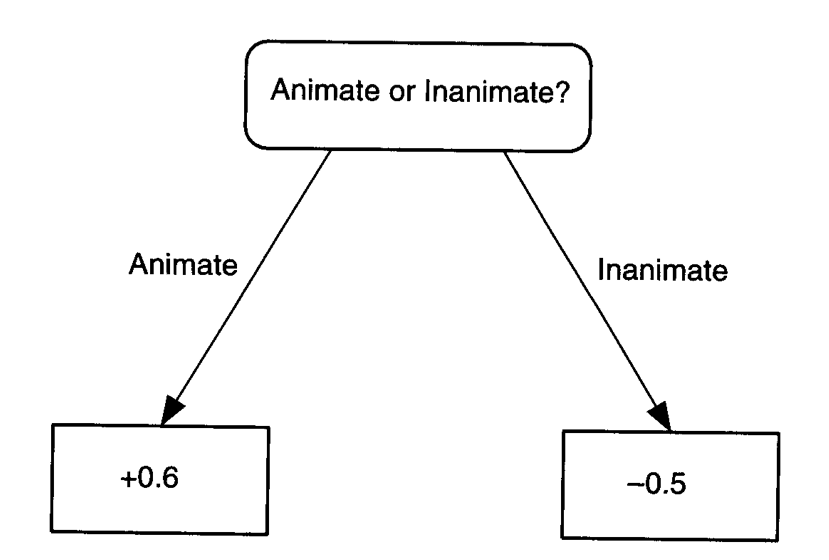
\includegraphics[width=70mm]{sources/images/TastyTree}\paragraph{}
    	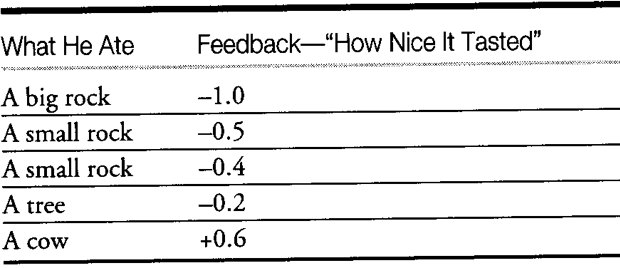
\includegraphics[width=70mm]{sources/images/TastyTable}
    	\caption{An example decision tree for a creature's experience eating objects \cite{:hc}.}
    	\label{fig:TastyTree}
\end{wrapfigure}

\noindent When the creature perceives information in its environment, it is stored in memory as a `belief'. The creature uses these beliefs to form opinions which alter their desires in-game to suit the player. To form opinions about its environment, the creature builds decision trees by looking at attributes that best categorise the knowledge into groups (see Figure \ref{fig:TastyTree} for an example). From these trees, a creature is able to make a prediction as to the outcome of performing a certain action. In the case of the example above, the creature would deduce that inanimate objects taste worse than animate ones, making it less likely to eat them in the future. 

The player also has the ability to reward or punish their creature when it performs certain tasks to further customise its learning. For example, if the player sees their creature eating a villager, they may choose to punish the creature to avoid the same thing happening in the future. This is accomplished using reinforcement learning. 

The creature is also able to learn by watching the player's actions and deducing what desire may have motivated the player. This dual approach stops the creature from falling into ``learning traps" by accidentally teaching the creature the `wrong' thing. For example, say the player wanted to teach their creature to avoid wolf creatures, but to be friendly to cow creatures. To do this, the player may punish the creature if it is friendly to a wolf creature. The creature may generalise from this punishment, and assume that it shouldn't be friendly to \emph{any} creatures, with no way for the player to correct the mistake. This combination of different techniques (or `representational promiscuity') help the agents to avoid many of the pitfalls associated with machine learning.

\section{Conclusion}

After researching different machine learning techniques, I feel that reinforcement learning, and more specifically Q-learning is the most appropriate method for my problem area. One of the key reasons for this is that reinforcement learning methods' use of the discount factor to take into account future rewards ensures truly optimal solutions, encouraging the system to act optimally from the start. Another reason for choosing Q-learning is that it excels in situations where the system has no prior knowledge of its environment (as with my game). Additionally, as my problem area is fairly limited with a relatively small number of possible action/state combinations per level, I will be able to store the state/action/Q-value data fairly easily in a table format. Had I chosen a more complex problem with thousands of possible states, trying to store every combination may be impractical.

Of the other methods I researched, I feel that decision tree learning is also suitable for my problem. However, I don't feel that using them for classification would fit my problem, as it would introduce unnecessary complexity; the obstacles that I'm using in my game are fairly basic, and trying to classify them would be unreasonable. Also, I don't feel that classification trees are suitable to the problem of learning an optimum route. Instead, I could use trees to dynamically map out the routes taken by an agent.

I have been made aware of a few issues which need to be addressed in system design. Firstly, I will need to make sure that my AI system doesn't learn the `wrong' thing, although this is unlikely as the system will not be influenced by the player at all. Another problem and one which may be difficult to work around is that of over-fitting (i.e. learning specific scenarios rather than generalised learning). However, as I am designing my system to learn to navigate specific levels, over-fitting is essentially the main aim. I may however be able to find a way to generalise the learnt knowledge so that it could be applied to other levels. 

Something I found particularly interesting about my research was the systems which incorporate the learning into the game itself, allowing the player to customise how the game behaves. While this is not appropriate for all genres of game, I feel that this could add an extra level of customisability for the player, and perhaps help the player to bond with the AI agents in a way that just isn't possible with traditional static AI systems.

Another interesting point which was emphasised by my research was that intelligence truly is ``in the eye of the beholder" \cite{:hc}. An AI system's behaviour is judged differently according to the observer; what may constitute strong and entertaining AI to one person could be completely frustrating for another. While this could be a pitfall of utilising machine learning in games, I feel that if implemented correctly, it can mean that an AI system can be tailored to match different levels of players.
	
\chapter{Choice of Tools}

I had to make sure that the applications and engines/code libraries that I chose would be suitable for their intended purpose before I started any serious development; trying to switch mid-way through the development process would undoubtably cause big problems were I to try and migrate the existing code later on.

\section{Programming Languages \& Game Engines}

My choice of language would not only have a big influence on the performance (and so the scale of the game and the features I could develop), but also the hardware that my game would run on. I initially planned to develop my project in Java as I was already comfortable using the language, and liked its cross-platform nature. I wanted to use the JMonkey engine for the game component, as it had powerful asset management, integrated GUI elements and applet integration to mention a few features. After carrying out a few simple tests however, I found it to be overly complex for my needs; it took a considerable amount of code to set up even a very basic scene. This isn't necessarily a fault of the engine itself, but rather of my choice to use 3D game engines in general; I had no need for the more advanced features such as complex physics and lighting etc. In addition, I didn't feel that 3D was particularly beneficial from an aesthetic point of view, considering my main inspiration was the classic 2D game Lemmings. I also had a few issues with a low framerate when adding many objects to the scene, which could cause me problems later on when I wanted to add many agents to the scene. Although this was likely due to my implementation rather than the engine itself, it highlighted to me the problems with developing in Java, and its lack of any memory management. Due to these points, I decided against trying to use a 3D engine and programming in Java.

My research eventually led me to Cocos2D: a 2D game engine originally written in Python, which has since been ported to many other languages including C++, Ruby and Objective-C. Using this engine opened up the possibility of developing my game for a mobile platform; something which greatly interests me (although admittedly, the JME does offer Android support). I felt that Cocos2D was particularly well suited to my project as it is well-established engine with a thriving community of developers making 2D games. It is also highly optimised for developing 2D games, with asset loaders, particle systems, and scene management to name a few of its useful features. It also comes bundled with two popular physics engines (Box2D and Chipmunk). Another benefit to using the Cocos2D engine is that it comes with libraries of code specifically optimised for games. For example, the engine comes with an alternative highly optimised collection class named `CCArray', which offers fast enumeration of its contents among other things. There is also a 'TextureCache' class which as the name suggests, caches textures in memory for quick access later. Cocos2D also offers sound support, integrated font rendering options, as well as some nice `automatic' (i.e. interpolatory) animation effects for moving objects smoothly on-screen. 

I decided to develop my project in Objective-C for the performance reasons that were outlined in my tests. One of the main benefits to using Objective-C over Java is that it offers powerful memory management features, and so affords the developer much more control over their application. Although this may not be so much of an issue with modern desktop systems, the amount of available memory in a mobile environment is still fairly limited. Objective-C is also comparable to C++ in terms of runtime `speed', due to the fact that Objective-C is essentially C (Objective-C is a strict subset of C) so any 'heavy lifting' code can be written in C if necessary to squeeze out the maximum performance. Objective-C also allows the developer to write code in C++ (called Objective-C++) if need be. Another benefit to using Objective-C is having the option to use Apple's \emph{Xcode} as a development environment, as well as the bundled \emph{Instruments} performance profiling tools to get detailed analysis of the program's runtime performance.

\begin{figure}[h!]
  \centering
    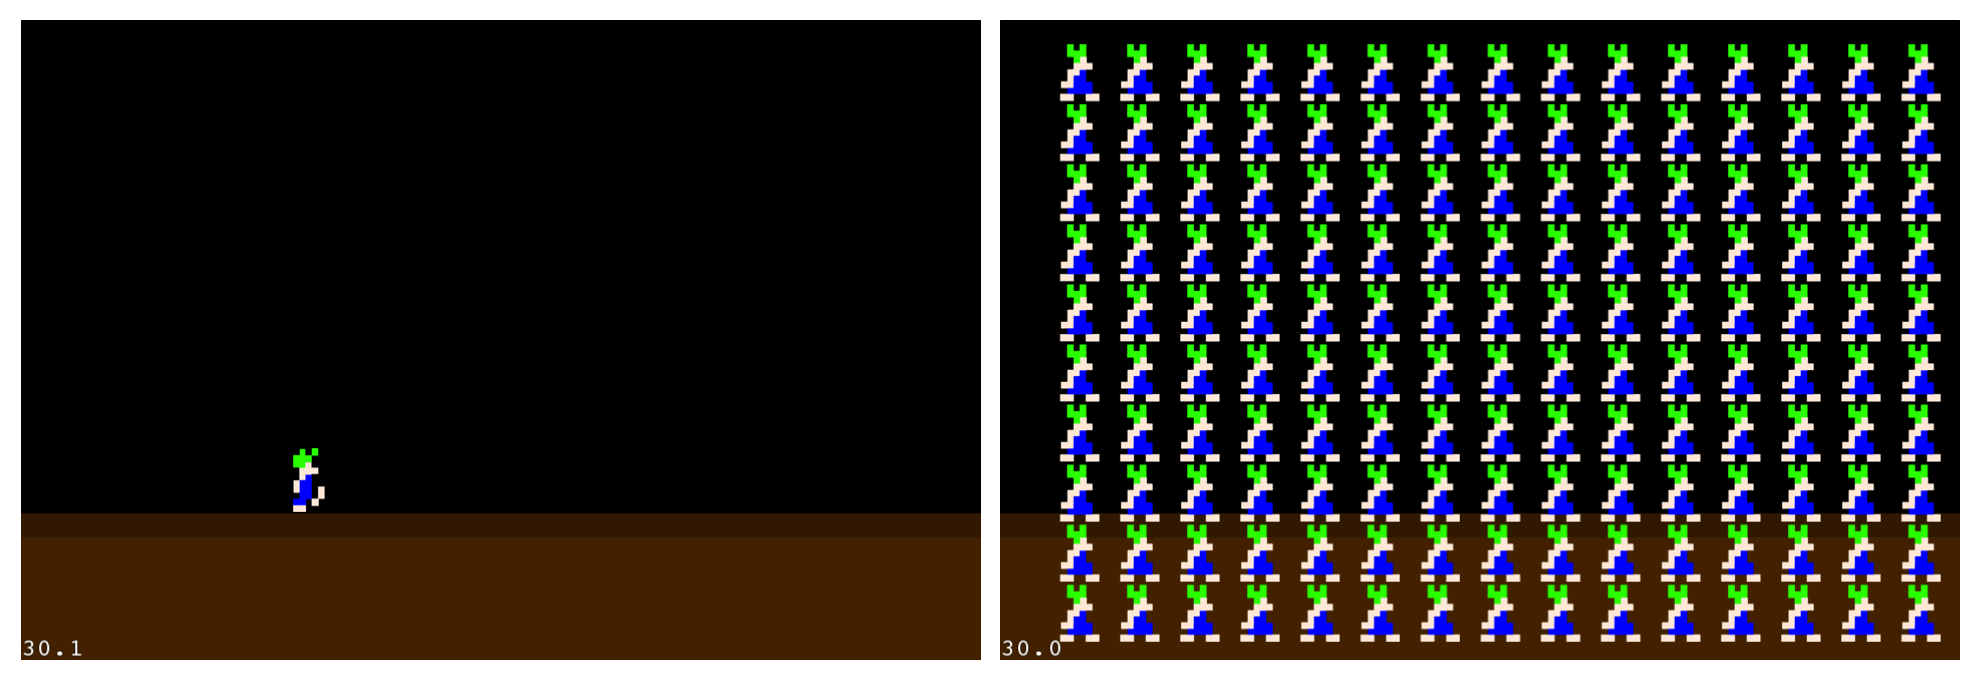
\includegraphics[width=140mm]{sources/images/InitialTests}
    \caption{Screens from my performance tests, both running at 30fps.}
    \label{fig:PerformanceTest}
\end{figure}

I carried out a few basic performance tests to see if there were any performance bottlenecks similar to the issues I had with JME. My first test was to add a single character to the scene, and animate it. My second test was to add more animating characters to see if there were any framerate issues; after adding 150 sprites, I was still achieving an impressive 30fps (see Figure \ref{fig:PerformanceTest} for screens). 

\section{Asset Production}

I also needed to create a variety of assets for my game (backgrounds, character sprites, menu items, fonts etc). The Cocos2D engine supports a variety of image file formats, including the lossless PNG format. For the creation of my graphical assets, I used an image manipulation program called \emph{Pixelmator} which exports to PNG as well as a number of other formats. I also needed to create texture atlases (or sprite sheets) in order to take advantage of Cocos2D's optimised sprite batch node feature (discussed more in the implementation section). For the fonts, I used a program called \emph{bmGlyph}, which is specifically developed for use with game engines that support the FNT file format.

\section{Version Control}

Using some form of version control system is a necessity in modern software development; it provides an easy way for multiple developers to collaborate on a single project (or even a single file) without causing file corruption. It is an invaluable tool for development teams, especially where developers are spread over different cities or even continents. It tracks all changes made throughout the development of the project, perhaps the most useful function of any version control systems as it not only allows the developers to see exactly what was changed (and by whom) in a project's history, but also means that were a mistake made, the project could easily reverted to an earlier state. Although I'm unlikely to experience any problems with file corruption as I'm the only one who will be contributing to the code-base, using a version control system still provides an incredibly useful way for me to not only track the progress of my project, but also as a way to incrementally back-up my project ensuring that any data loss is recoverable.

There are a variety of different source control systems available, such as CVS, Subversion, Mercurial and Git. I decided to use Git as the version control system for my project as it is widely supported by many IDEs and other version control management software. I also generally prefer Distributed Version Control Systems (DVCS) as opposed to centralised systems because I like the freedom DCVS systems give you in terms of being able to work on a project without the need for an internet connection. DVCS systems also provide more security as each user has a backup of the entire system. However, this could take up an inordinate amount of storage space were I working with many binary files (for example Adobe Flash files), in which case using a DVCS would be unsuitable. I will be using a Git server hosted by GitHub to store the source code and documentation for my project. 

\section{Project Management}

To manage the progress of my project, I used a web-based application called ProjectPier which I installed on my web server so could be accessed from anywhere. Using this system, I split my project into a number of `task-lists' for each component in my project's development; for example: asset production, game development, AI development, testing, etc. I also added milestones to my project to mark specific targets that I wanted to achieve by certain dates. Using this system, I could add individual tasks that needed to be completed, deadlines (or 'milestones') to mark specific targets in the development of my project. I could also use the system to create a wiki for my project containing useful information. 



%
% New part
%

\part{Planning}{This section covers the process of designing my system, from the initial concept art and art direction, to the system functionality modelling.}

\chapter{Artwork}
	
The first task I carried out when designing my game was to create some initial artwork. Not only would this help to define the look and feel of the game, but it would also help me to visualise how the levels could be structured, which would give me more of an idea as to exactly what kind of functionality was feasible. In addition to logos and some initial art direction, I also created the initial art for the agents, some sample screen artwork and some level designs.
	
\section{Logo Design}
	
\begin{wrapfigure}{r}{0.55\textwidth}
  \centering
    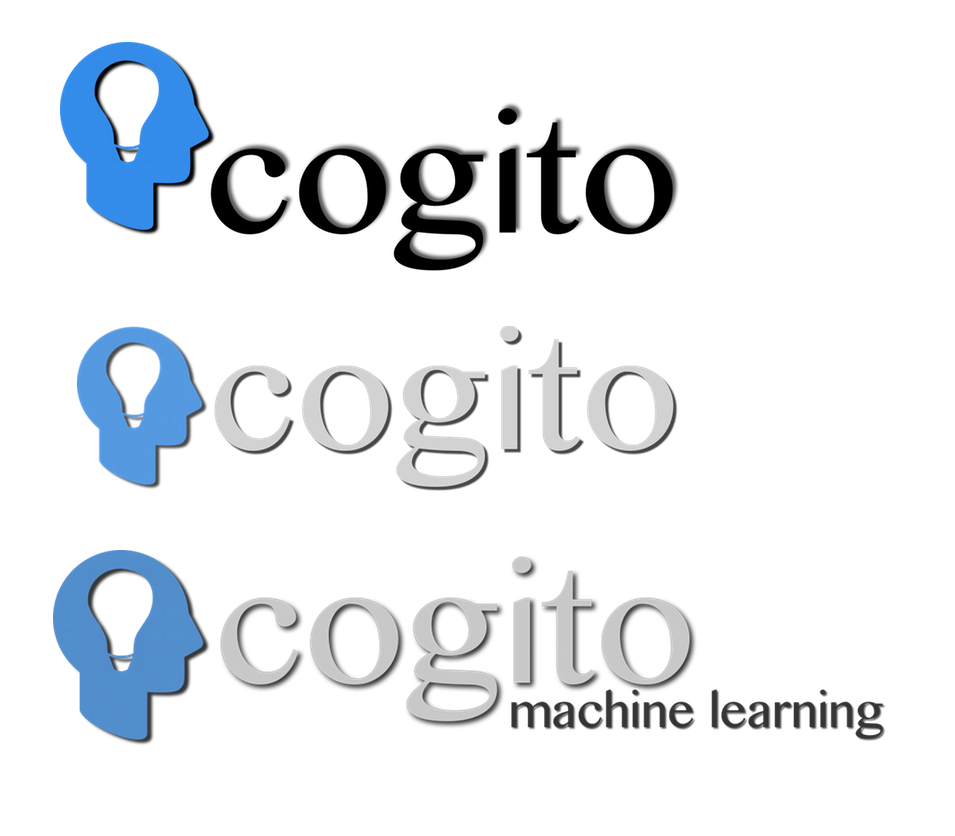
\includegraphics[width=65mm]{sources/images/cogito_logo1}
    \caption{Iterations of My Logo Design}
    \label{fig:Logos}
\end{wrapfigure}
	
I went through a few different iterations of logos (see Figure \ref{fig:Logos}). I final settled on a blue/white/grey colour scheme. I wanted the art style to be clean and unobtrusive, so didn't want to use a lot of bright colours. For this reason, I went for a mainly monochromatic colour scheme, with the blue used sparingly for emphasis. I would use this colour scheme throughout my game for the menu, levels, characters and any other screens.

\section{Game Design}

After settling on a colour scheme and basic art style, I then went about creating some mockups of various screens that I would be using in my game (see Figure \ref{fig:ScreenMockups}).
	
\begin{figure}[h!]
  \centering
    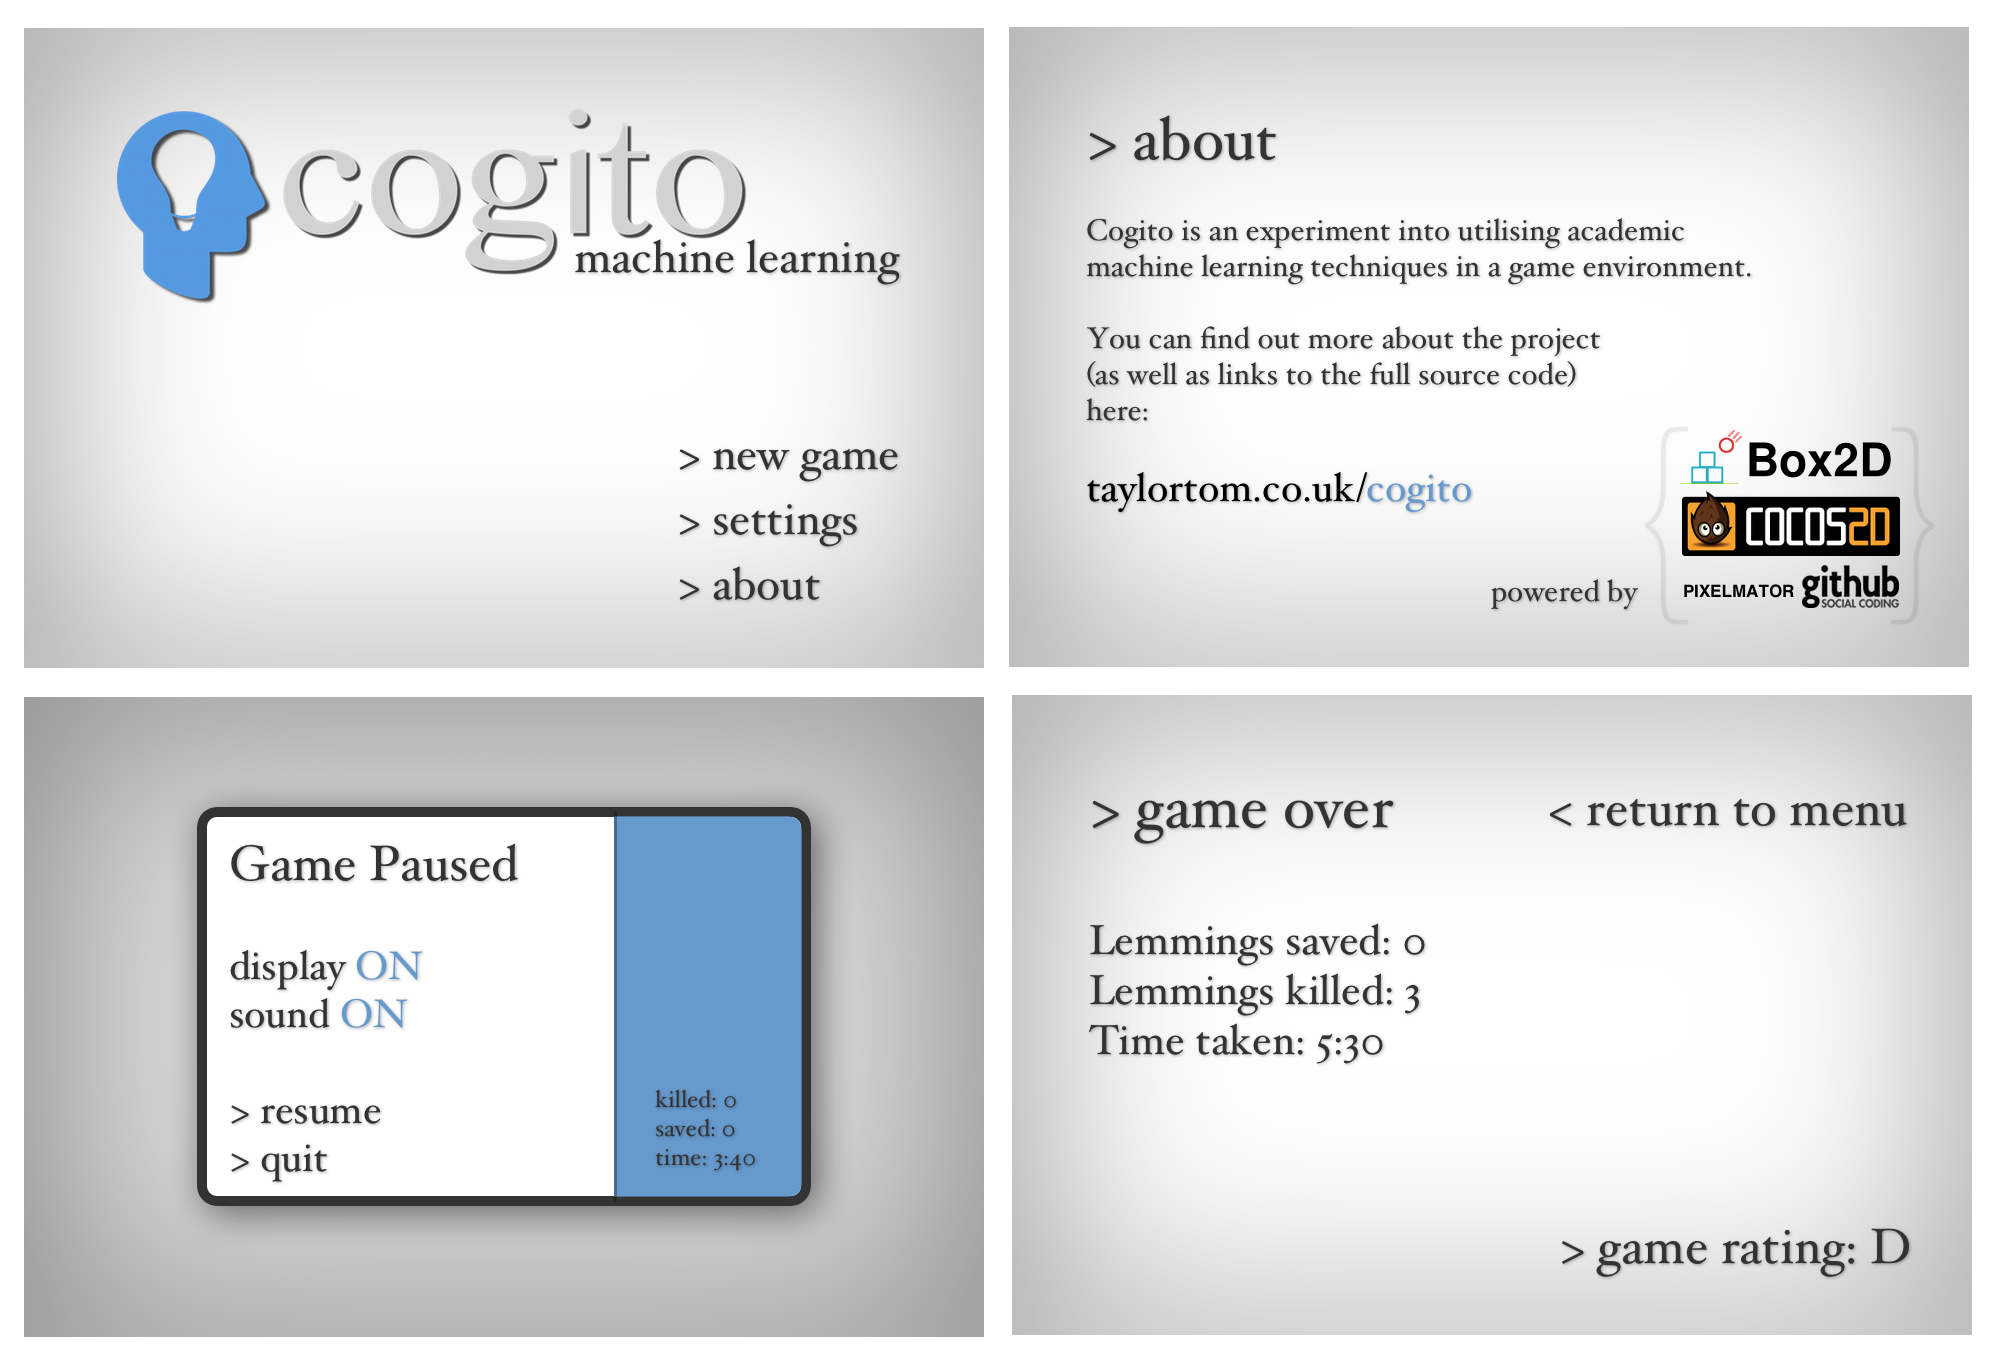
\includegraphics[width=140mm]{sources/images/Screens}
    \caption{Initial Screen Mockups and Art Direction}
    \label{fig:ScreenMockups}
\end{figure}

I also created a basic level design to give me more of an idea as to how a level might look. The idea of this was to get more of an idea of exactly how I might implement the level later; how the agents might transition between the different levels etc. I also decided to split the level into a number of `nodes' (visible in Figure \ref{fig:LevelDesign}). This would serve to simplify the agent's navigation, and is a similar idea to navigation meshes used in many games.  

\begin{figure}[h!]
  \centering
    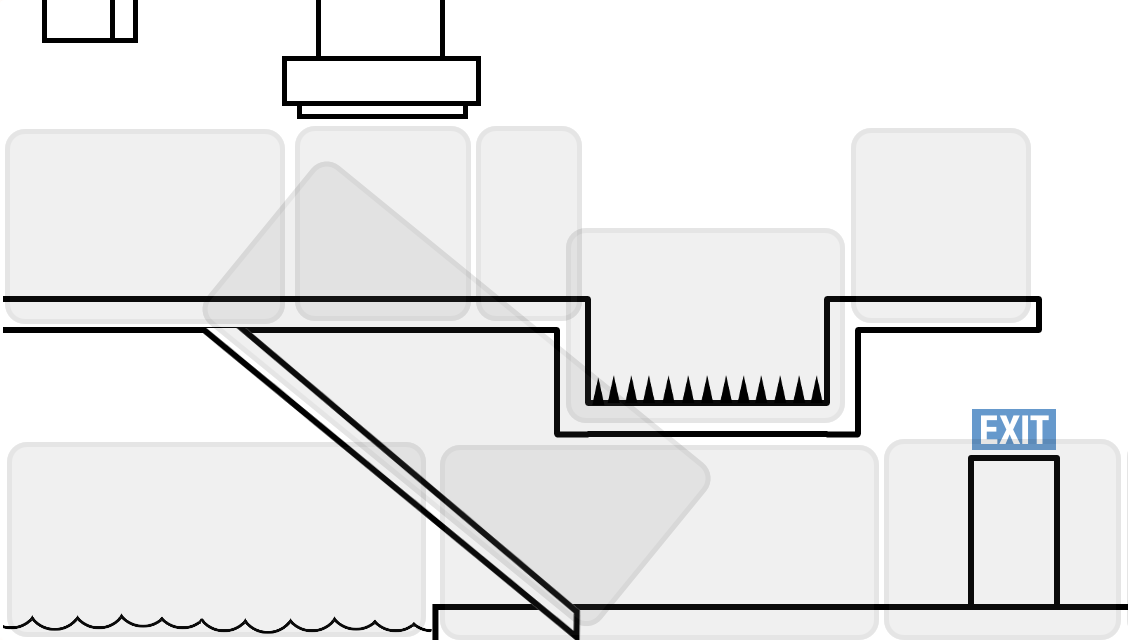
\includegraphics[width=120mm]{sources/images/LevelDesign}
    \caption{Initial Level Design}
    \label{fig:LevelDesign}
\end{figure}
	
\section{Sprite Design}
		
I took a lot of guidance from the original sprite style and animation used in the original Lemmings game (see Figure \ref{fig:LemmingWalkerSprites}). I decided to stay with the simple 8-bit art style for the sake of simplicity.
	
\begin{figure}[h!]
  \centering
    
\includegraphics[width=80mm]{sources/images/lemmings-walker-sprites}
    \caption{The Original Lemming Walking Animation \cite{Marsh:vn}}
    \label{fig:LemmingWalkerSprites}
\end{figure}
		
Using the above as inspiration, I created the walking animation frames, as well as the other animations required in my game (walking with helmet, open/use umbrella, floating, death). I used my chosen colour scheme for the agents to fit in with the rest of the art style.
		
\begin{figure}[h!]
  \centering
    
\includegraphics[width=60mm]{sources/images/Final}
    \caption{Final designs for agent sprites}
\end{figure}

I later added a faint outline to the agents, as I found when testing the game that the they became indistinguishable against the white background.
	
\begin{figure}[h!]
  \centering
    
\includegraphics[width=60mm]{sources/images/Lemming_walk_anim}
    \caption{The Final Walking Animation}
\end{figure}
	
\chapter{System Design}

After creating initial artwork, I created a `brief' to give a more concrete outline of the functionality for my game. From this, I could then structure it in into logical interrelated classes. I split my game into three logical components: the menu structure, the game component, and the AI system. I outline each briefly in this section.

\section{Menu}

Rather than start the game start as soon as it is loaded up, I wanted to implement a simple menu system. My menu needed to obviously contain a link to a new game screen, as well as links to the game instructions and an `about' screen. My menu needed to be uncluttered, and ideally have one `level' (i.e. no nested menus). Included in the menu component were two screens: the instructions screen to give basic information about playing the game, and the `about' screen to give a bit of background information about the project.

\section{Game}

My `game' component needed to be able to load and transition between different scenes (i.e. menu and instructions scenes). It also needed to load the external game assets and level files and build the levels from these. It also needed to be able to animate these assets. I also needed to control the actual running of the game (i.e a game timer, pausing/resuming and exiting). I needed to implement some way to add and remove the characters, and detect when the game has ended. Finally, I wanted to implement a game over screen with a game rating to indicate to the player how well they had done. I also needed some way to pause and exit the game.

\subsection{Lemming Functionality}

The lemming characters needed to be able to move around the level, change state, have basic collision detection, play basic animations and to be able to detect if an end condition has been reached.

\section{AI System}

The AI system was required to generate a list of actions available to the agents, and detect when an agent has reached a `decision point'. The system also needed to be able to dynamically create and maintain a knowledgebase of routes using: shortest route, decision tree and reinforcement learning (Q-learning) methods. The agents should have a `learning mode' which is used to form the knowledgebase. This knowledgebase should then be used to generate an optimum policy (or route).

\section{Class Diagrams}

I created some initial class diagrams to specify how I intended to design the system. These classes show their intended functionality, and how they relate to other classes in the system. 

\subsection{Layers}

The layers contain the actual game content, such as background sprites, the character sprites, menu items, text labels etc. These are the initial specifications for the layers in my game (Figure \ref{fig:Layers}).

\begin{figure}[h!]
  \centering
    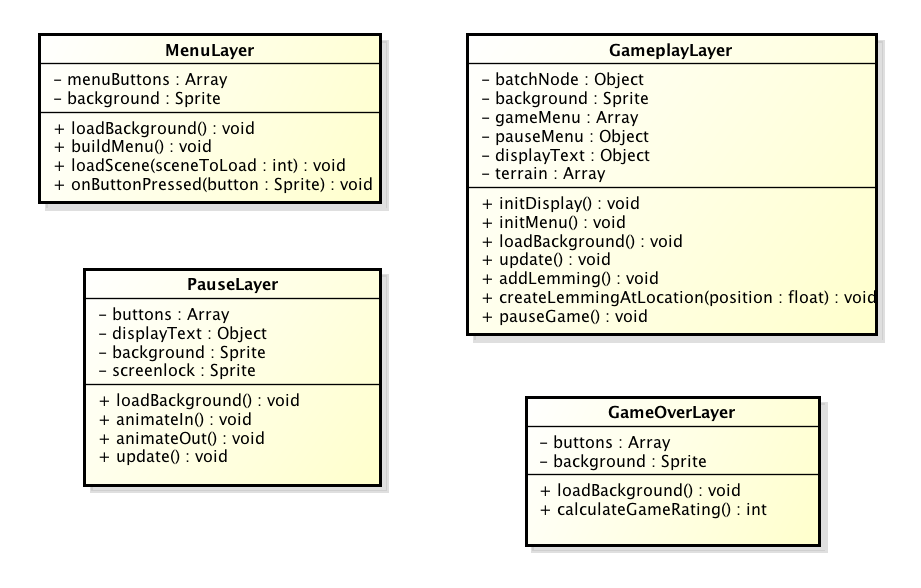
\includegraphics[width=140mm]{sources/images/Layers}
    \caption{The `Layers'}
    \label{fig:Layers}
\end{figure}

\subsection{Singletons}

I intended to use a number of classes using the singleton design pattern to manage the shared data in my game. I initially decided to use LemmingManager and GameManager singletons, although I ended up adding more in my final system (Figure \ref{fig:Singletons}).

\begin{figure}[h!]
  \centering
    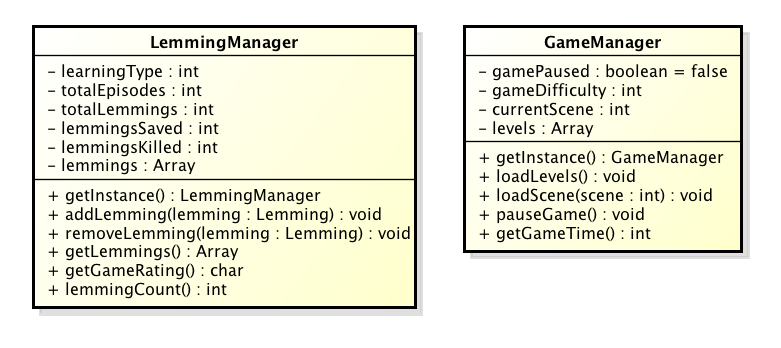
\includegraphics[width=120mm]{sources/images/Singletons}
    \caption{The Singletons}
    \label{fig:Singletons}
\end{figure}

\subsection{GameObjects}

I planned to create a base class called `GameObject' which would be inherited by all of the game objects I would be using in my game. Objects such as the agents and the level terrain (Figure \ref{fig:GameObjects}).

\begin{figure}[H]
  \centering
    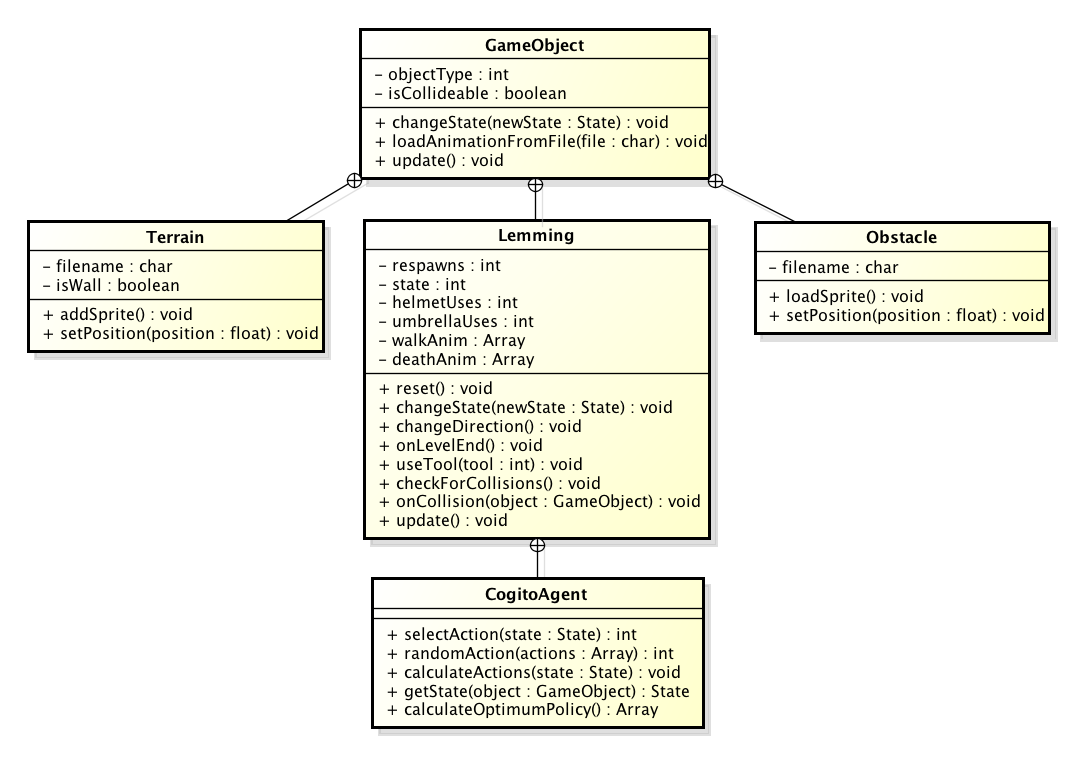
\includegraphics[width=150mm]{sources/images/GameObjects}
    \caption{The Game Objects}
    \label{fig:GameObjects}
\end{figure}
	
\newpage
	
\section{Agent States}

I also created a basic state diagram to map out the intended states for my game characters (see Figure \ref{fig:LemmingFSM}).

\begin{figure}[H]
  \centering
    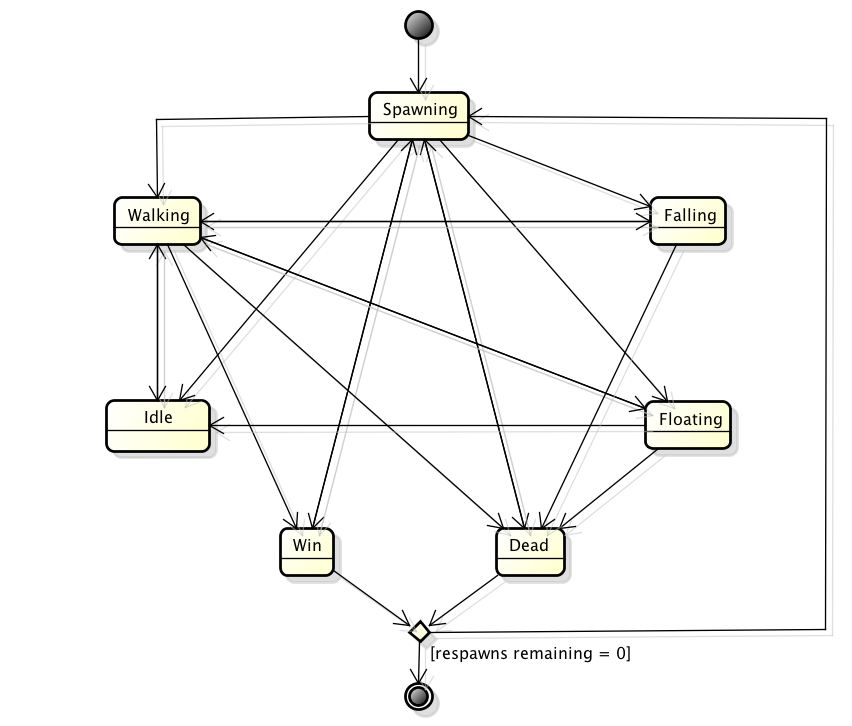
\includegraphics[width=120mm]{sources/images/LemmingStatemachine}
    \caption{Character States}
    \label{fig:LemmingFSM}
\end{figure}
	
\section{Scheduling}

I created a schedule for the development of my project. In it, I outlined the major processes involved in the development stage: planning/research, game development, AI development and testing/debugging. I then split each stage into a series of sub-tasks, such as `asset production' and `research frameworks'. See Appendix A for my initial project schedule.

\section{Contingency Plan}

To avoid any problems arising due to data loss, I was sure to make sure that I had sufficient back-ups of all components of my project. The code itself was maintained using git and stored on a Github server. This meant that I always had a complete history of my project online. Additionally, I created a weekly archive of my code and uploaded it to a cloud storage service. As the source files for my graphical assets were very large in size, I decided not to store them on the git server, and instead kept them locally on my development computer, also backing them up to a cloud storage service. I also made weekly backups of my computer to an external hard-drive.

As I was developing my project alone, it was difficult to create a contingency plan to account for a loss of development time (due to illness etc.). My solution was to increase my time-estimates for each development state by 20\%.
	
\section{Social, Legal, Ethical and Professional Issues}

When designing my game, I had to consider a number of social, legal, ethical and professional issues to ensure that my product and its development complied to any applicable laws and ethical standards.

\subsection{Intellectual Property}

All of the intellectual property used in my game is my own, with the exception of the Cocos2D framework which I used. I have cited that I have used the engine in the game itself on the `about' screen. I have also included a copy of the relevant license in the source code. The engine is published under the MIT licence, which states that it is free to use in proprietary software provided that all copies of the software also include a copy of the license. A big benefit of the MIT license is that software which uses MIT-licensed code has no obligation itself to be published using the same license, and can be completely closed-source.

\subsection{Copyright Law}

In order to ensure that my product complied with copyright laws, I decided to create all assets needed myself. This ensured that I didn't need permission from any third parties prior to developing/releasing my product. All of the assets such as the backgrounds, logos and animations have been created by me solely for the purpose of this project.

\subsection{The Data Protection Act}

I don't store any personal data about the user in my game, so there are no issues regarding the Data Protection Act. The only information I collect is data regarding the agent's learning in the game, which is not transmitted to any source, but is simply used within the game to provide some basic stats about the system.

\subsection{Ethical Issues}

As I carried out my usability tests with the help of human subjects, I made sure that the subjects were kept completely anonymous and all information with regards to them confidential. There was no need for my to store any personal data about them, so this didn't really present an issue.



%
% New part
%

\part{The Product}{This section gives a detailed description of my actual product, along with relevant screenshots.}

\section{The Menu}

Upon loading the game, the player is presented with the main menu screen. From the menu, they can start a new game, view game instructions, view basic game stats and view some other useful information about the game on the `about' screen. The instructions and stats screens contain multiple pages of information, which can be navigated using the onscreen buttons (see Figure \ref{fig:FinalScreens}).

\begin{figure}[h!]
  \centering
    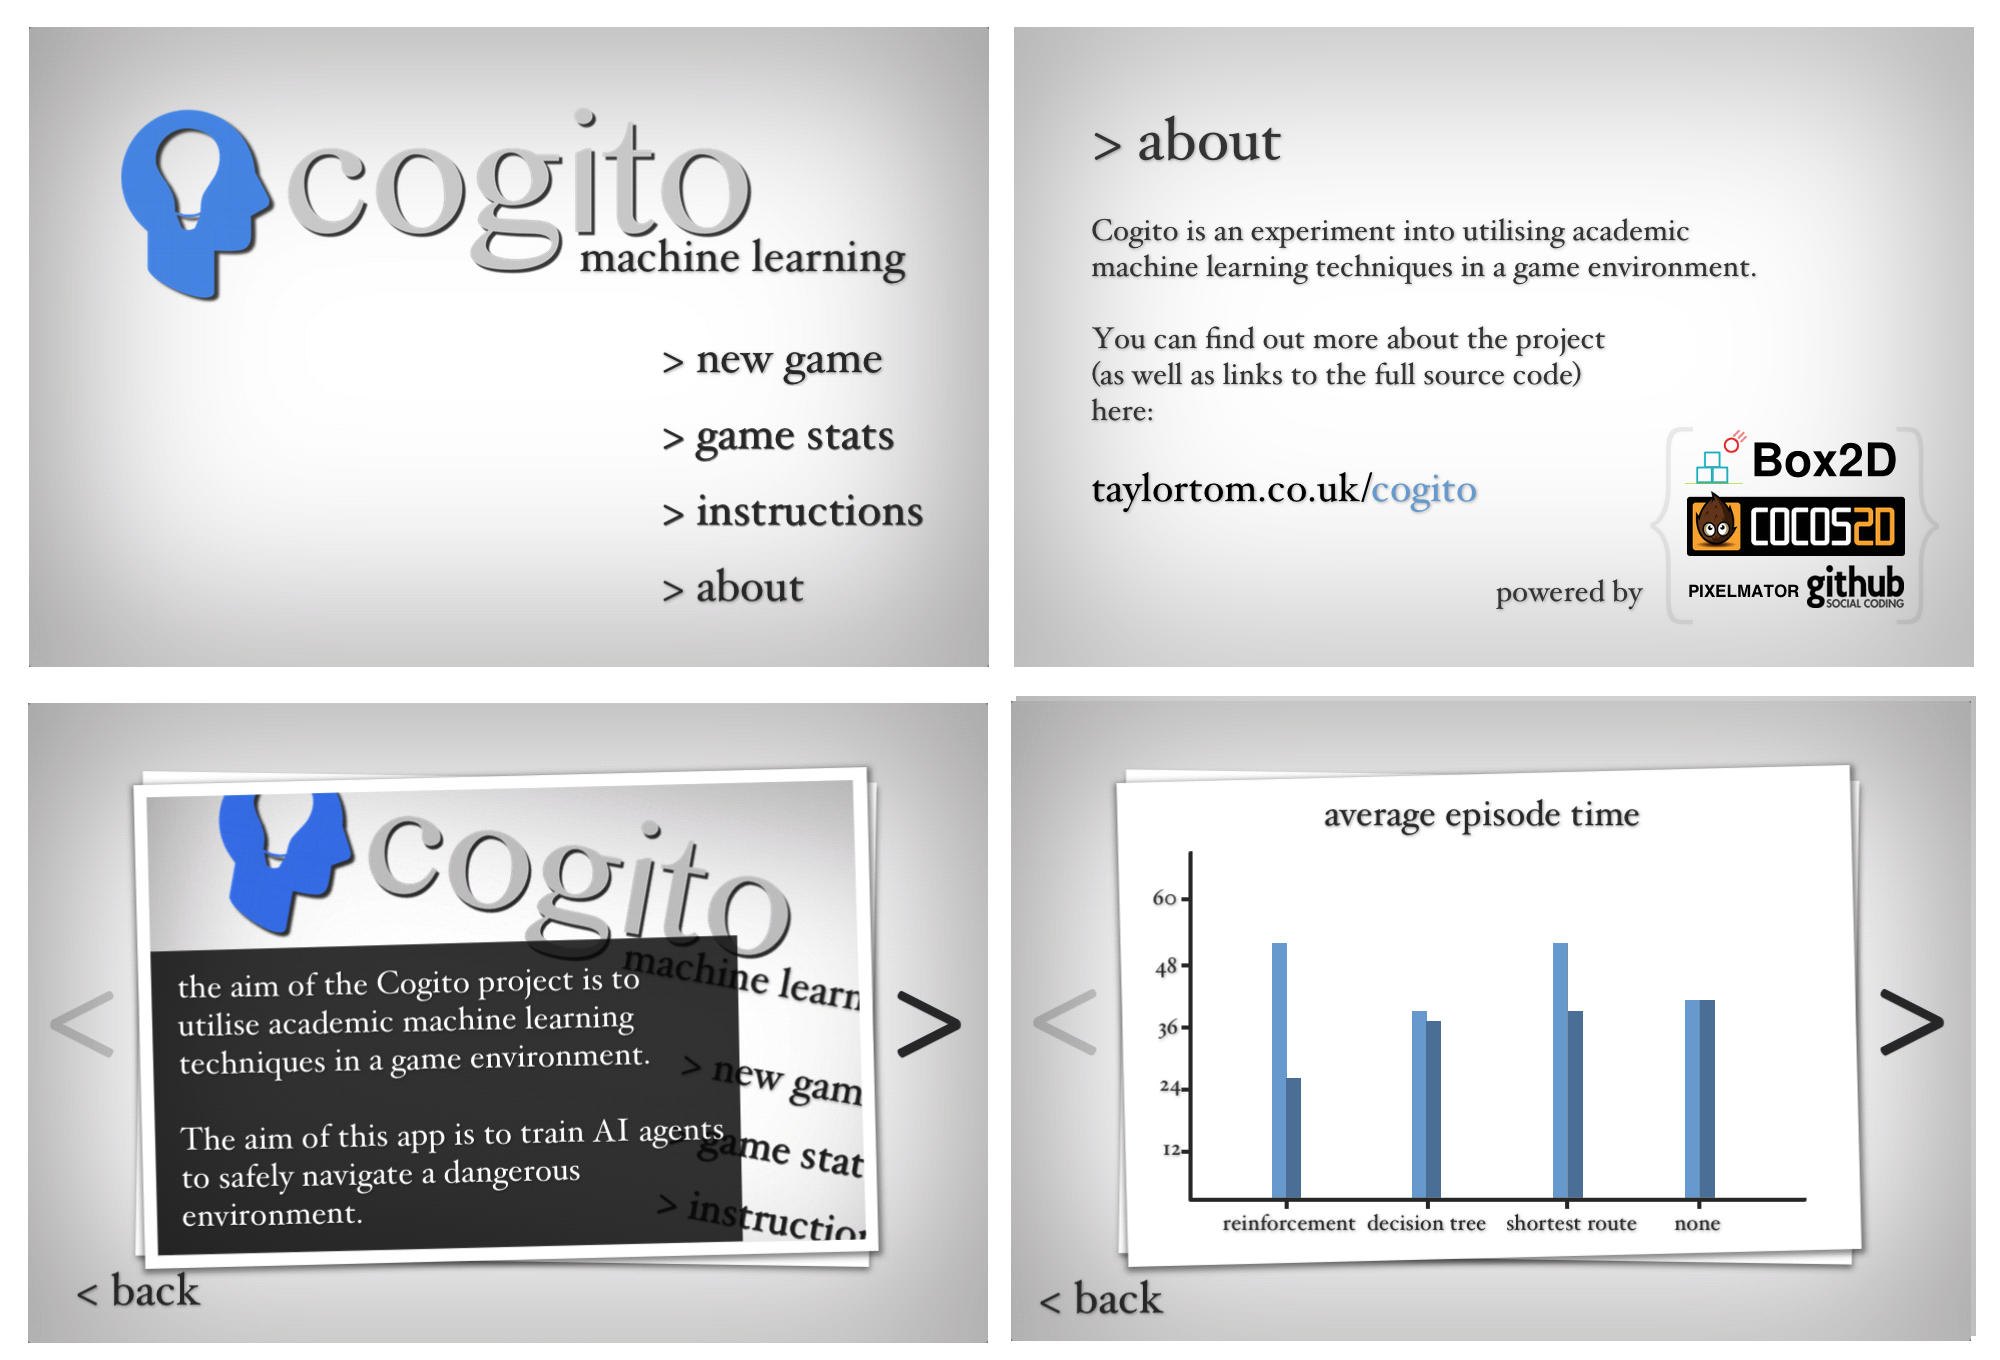
\includegraphics[width=120mm]{sources/images/FinalScreens}
    \caption{Main Menu and Related Screens}
    \label{fig:FinalScreens}
\end{figure}

\section{Starting A Game}

\begin{wrapfigure}{r}{0.55\textwidth}
  \centering
    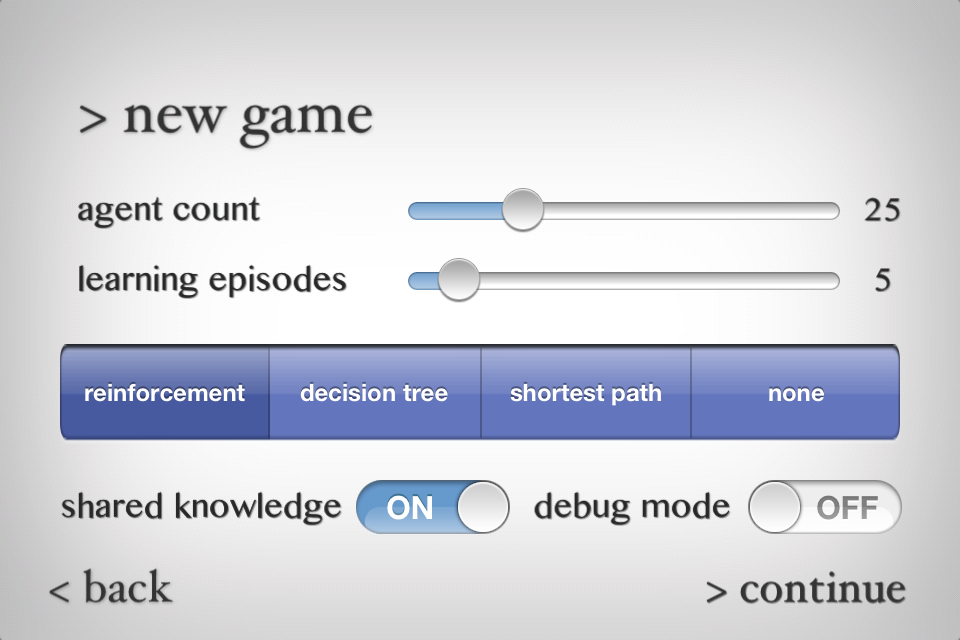
\includegraphics[width=70mm]{sources/images/Screen_NewGame}
    \caption{New Game}
    \label{fig:NewGame}
\end{wrapfigure}

Before beginning a game, the player is presented with a new game screen allowing various game parameters to be tweaked (see Figure \ref{fig:NewGame}). On this screen, the player can move the sliders to adjust the number of agents and learning episodes in the game as well as the learning type. There is also the option to enable a shared knowledgebase to speed up learning (a feature currently only available when using reinforcement learning), and an option to play the game in debug mode. In debug mode, the game displays the (usually invisible) `decision nodes' and the game framerate.

\section{Playing The Game}

When the new game parameters are confirmed, a level is chosen at random and the game begins. The agents begin to spawn into the level at the top of the screen, and begin to traverse the level, forming a knowledgebase as they go. 

The agents begin in `learning mode' and navigate the levels randomly (which speeds up the learning process). While navigating the level, the agents will come to various decision points (trapdoors and the end of platforms) where they must decide from a number of possible actions (from: left, left with helmet, right, right with helmet, equip umbrella, down - which are available depends on the current state). Two tools aid the agents to overcome obstacles: the helmet to protect from the stampers, and the umbrella to protect from big drops. Based on their actions, the agents will eventually reach an end condition: either falling victim to an obstacle (water, stamper, or a big drop) resulting in instant death, or reaching the level exit - both signify the end of the learning `episode'. This process repeats until all learning episodes have been completed, at which point the agent spawns for a final time, distinguishable by the `!'  or `?' over the agent's head (highlighted in Figure \ref{fig:GameScreen}). The question mark is used in the decision tree/shortest route methods, and signifies that an agent was unable to find safe route in the allotted learning episodes. In this final episode, the agents use what they have learnt to create an optimal route to the exit.

\begin{figure}[H]
  \centering
    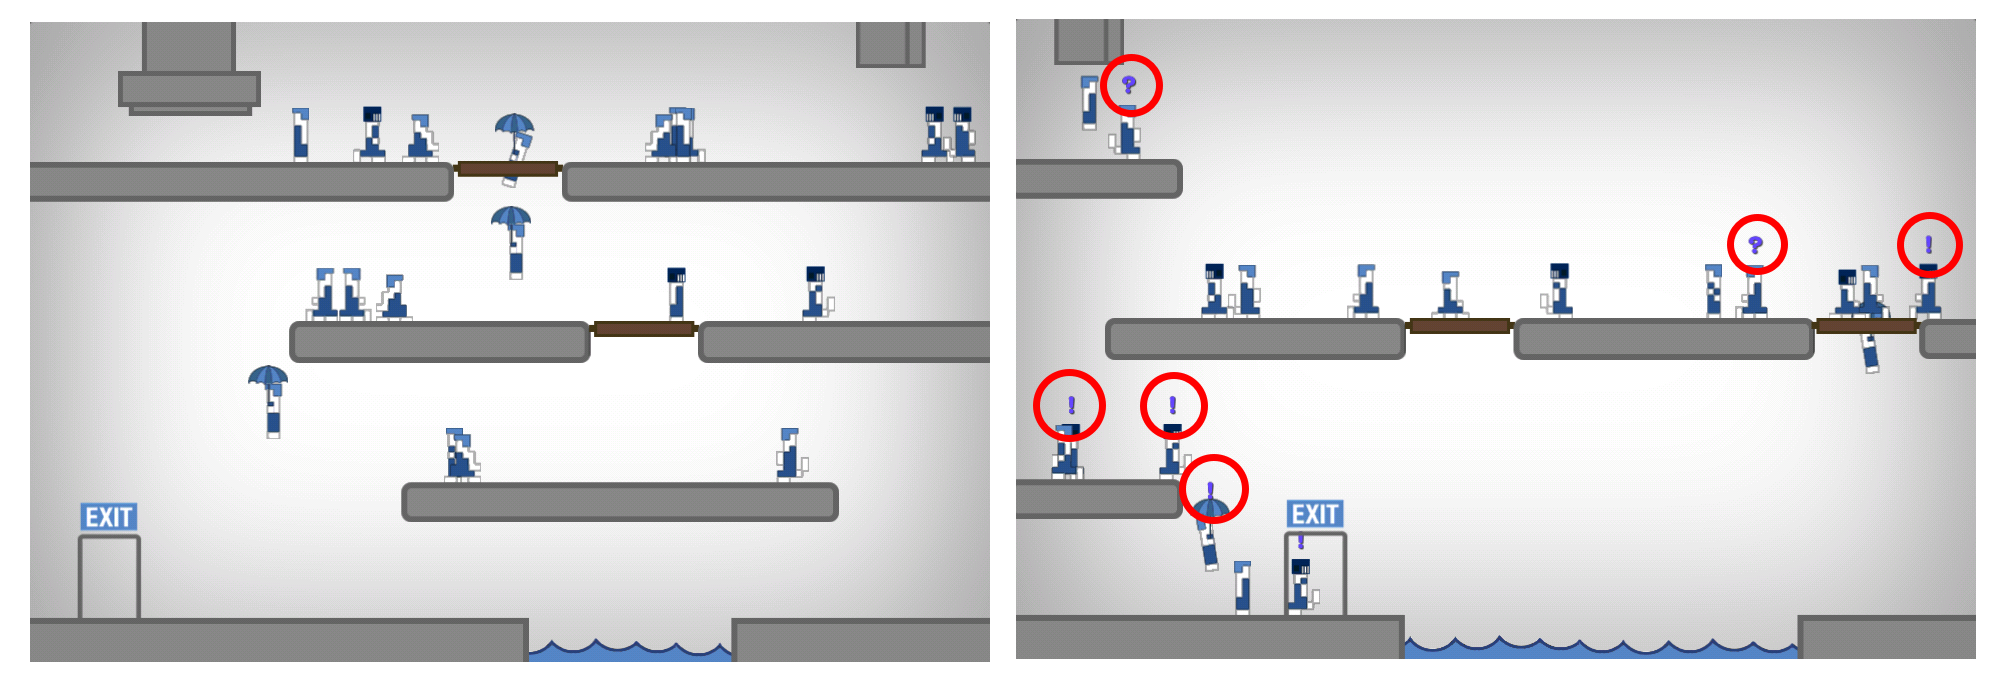
\includegraphics[width=130mm]{sources/images/Screen_Game}
    \caption{In-game Screenshots}
    \label{fig:GameScreen}
\end{figure}

When all agents have completed this final episode, the game ends revealing a game over screen which displays some game statistics and a rating of the agents' performance (see Figure \ref{fig:GameOver}).

\begin{figure}[H]
  \centering
    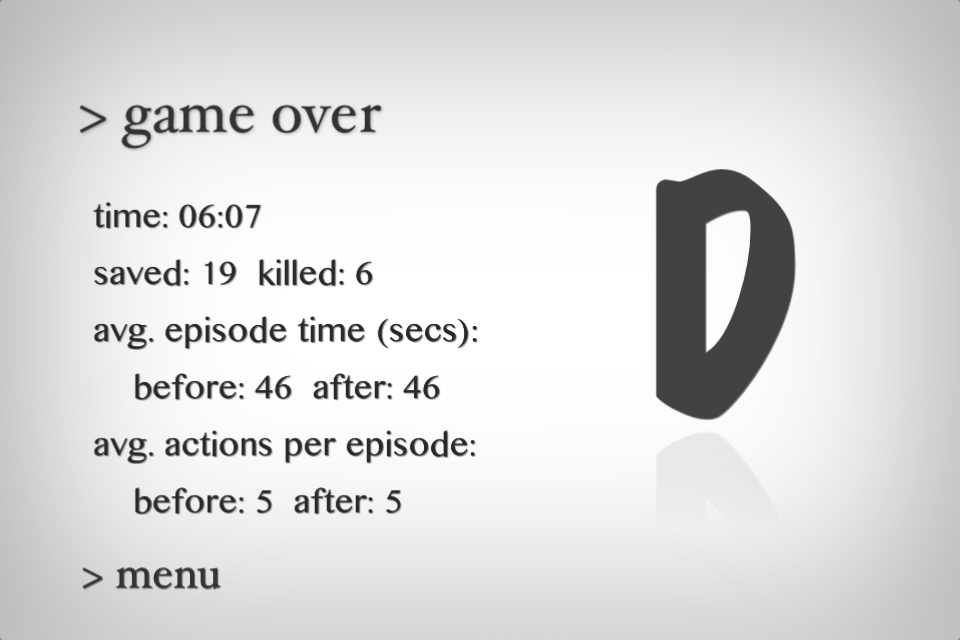
\includegraphics[width=65mm]{sources/images/Screen_GameOver}
    \caption{The Game Over Screen}
    \label{fig:GameOver}
\end{figure}

\paragraph{Pausing the game:} The game can be paused by simply touching the screen while in-game. Doing this brings up the pause `HUD' which displays useful data about the current game (see Figure \ref{fig:PauseScreen}). It also has the option to quit the game. \\

\begin{figure}[H]
  \centering
    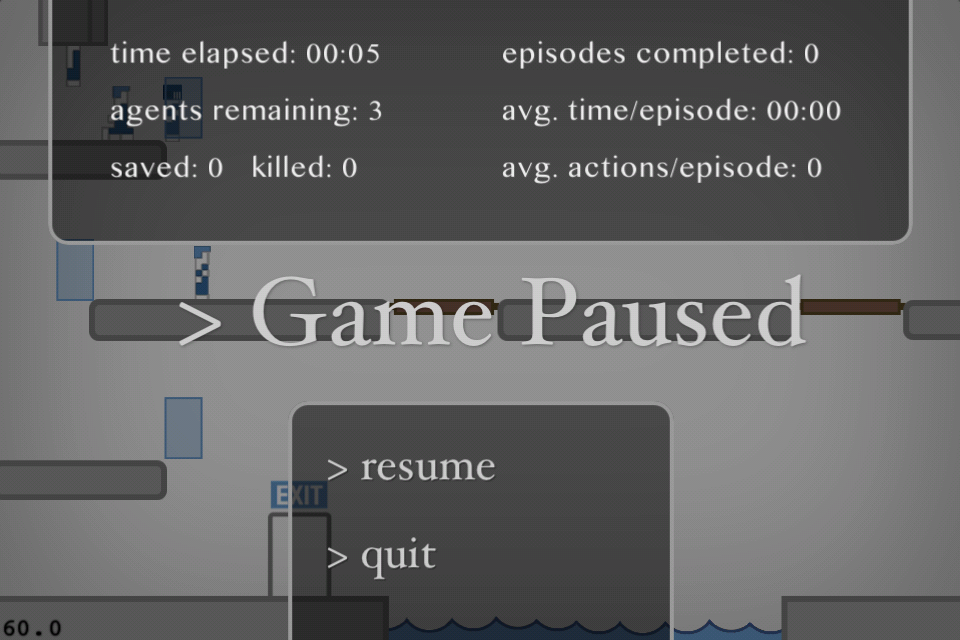
\includegraphics[width=70mm]{sources/images/Screen_Pause}
    \caption{The Pause Screen}
    \label{fig:PauseScreen}
\end{figure}

%
% New part
%

\part{Implementation}{This section covers the process of actually implementing my system, problems that I was faced with, and how I solved them.}

\chapter{Coding Practices and Structure}

When writing the code for my project, I tried to stick to standard code formatting conventions and use standard design patterns where possible to ensure that my code was easily readable to others. 

\subsection{Commenting}

I have used a universal comment format in my program to improve readability. I also avoid commenting variables wherever possible by self-descriptive variable names.

\begin{lstlisting}[label=some-code,caption=Comment Formatting]
//
//  File name
//  Project name
//
//  Class description
//
//  DD/MM/YYYY: Created class
//

/**
 * Method description
 * @param any parameters
 * @return the returned objects
 */
 \end{lstlisting}

\subsection{Methods}

The format of my method headers is fairly standard. However, I prefix all method parameters with an underscore as it helps to clarify which variables in a method are parameters if quickly scanning the code.

\paragraph{}-(void)addLemming:(CCSprite*)\_lemmingToAdd;


\subsection{Singleton Classes} 

I made a lot of use of the singleton design pattern throughout my project to create various `manager' classes to deal with the shared data in my system. A singleton class is a special kind of class which only has one instance; calling a singleton instance will always return the one instance of the class, regardless of which class called it. The major benefit of using the singleton pattern being that you only need to store the data in one location, which can then be accessed by any class anywhere in the program (provided that the access to the data is restricted to a single thread at a time to avoid concurrency issues). My LemmingManager class which handles all of the agents in the game is an example of where I have used this pattern. It holds the only list of the characters in the game, and contains the functionality to add and remove lemmings among other things.

\subsection{Constants and Datatypes} 

I put all of the read-only `constant' variables (framerate, reinforcement learning rewards etc.) into a file so that they are easily be found and modified. It also meant that I only needed to alter the values in one place, rather than having to search every source file. Each constant follows the standard naming convention (i.e. starting with a "k"), a legacy feature from the pre-Mac OS X days, possibly back when the Mac OS was written mostly in Pascal. 

I also created a similar file which contained many common datatypes which I would be using in my game, such as machine learning type, terrain type, character state, game rating and so on. As with the constants, this meant that I could keep all of the needed datatypes in a common location for easy access.

\subsection{Utility Methods} 

I created a Utils class with some static-access `utility' methods which I would be usng a lot in my game (random number generation, enumeration-to-string conversions, timestamp generation etc.). I created a separate class with these methods to not only cut down on the amount of code that I had to write, but also so that I would only need to fix any bugs with the code in one place, rather than having searching every source file. 

\subsection{Class Listing}

Below is a list of the classes used in my program. More detailed information can be found in the HTML documentation on the resources disk (see Appendix E).

\begin{figure}[H]
  \centering	
	\begin{tabular}{l|l|l|l|l}
		\hline
		\textbf{Layers} & \textbf{Scenes} & \textbf{Objects} & Singletons & \textbf{Misc} \\ \hline
		AboutLayer & AboutScene & GameObject & AgentStats & Constants \\ 
		BackgroundLayer & GameScene & Lemming & DataManager & Datatypes\\
		GameOverLayer & GameOverScene & CogitoAgent & GameManager & Utils \\
		GameplayLayer & InstructionsScene & DecisionTreeAgent & KnowledgeBase \\
		InstructionsLayer & StatsScene & QLearningAgent & LemmingManager \\
		MainMenuLayer & StingScene & ShortestRouteAgent & \\
		NewGameLayer & MainMenuScene & Obstacle & \\
		PauseMenuLayer & NewGameScene & Terrain & \\
		StatsLayer &  & Level & \\
		StingLayer &  & Route & \\
		TerrainLayer &  & Slide & \\
		 &  & GraphSlide & \\
		 &  & SlideViewer & \\
		 &  & State & \\
		 &  & QState & \\
		 &  & TreeState & \\
		
	\end{tabular}    
	\caption{Classes Used in Cogito}
	\label{fig:ClassList}
\end{figure}

\chapter{Game Component}
		
\section{Code Structure/Features}

My first task was to create the underlying game component. As I was using the Cocos2D engine, a lot of the very low-level functionality had been taken care of such as the direct OpenGL ES calls needed for loading and binding textures. However, I still needed to take care of loading levels, adding objects, game characters, animating characters etc.

\subsection{Cocos2D} 

The Cocos2D framework comes with a very useful code library with various optimisations and utility methods which I made use of when implementing my game. There a number of different base classes which can be used and take care of a lot of the very low-level functionality such as OpenGL API calls. These classes are organised into a hierarchy (see Figure \ref{fig:Hierarchy}). 

\begin{wrapfigure}{l}{0.5\textwidth}
  \centering
    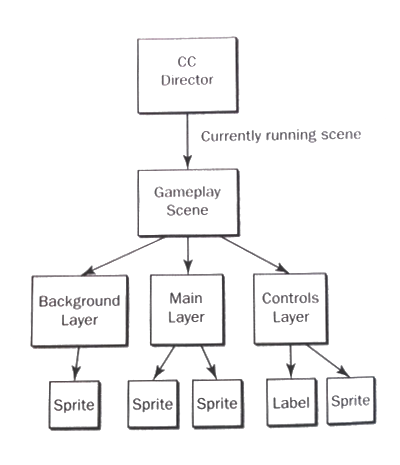
\includegraphics[width=70mm]{sources/images/Cocos2DHierarchy}
    \caption{Cocos2D Scenes, Layers and Sprites Hierarchy \cite{Strougo:2011ys}}
    \label{fig:Hierarchy}
\end{wrapfigure}

At the highest level is the CCDirector class which, as one would expect, controls the running of each individual `level' in the game (called scenes). In addition to actual game levels, scenes can also be menu systems, game over screens and so on. Each scene consists of one or more layers which contain the actual game objects (for example background images, any level terrain and the game characters). The game objects themselves (known as sprites) are at the bottom of the hierarchy and are just essentially an image with no real functionality by default. 

Cocos2D also includes a number of other useful features, such as the ability to add `transitions' in between scenes, and the CCAction class which allows the programmer to easily add an animation to sprite objects by simply specifying a start and end position and a duration. The class then creates an animation by interpolating between these two points. I use these actions in a number of places throughout my game, from animating the main menu items, switching graphs in the game stats screen, moving the agents in the game, and animating the game's pause menu. Cocos2D also includes some highly optimised data structures such as the CCArray class, a collection class which has been optimised for high-performance, with features such as fast enumeration.

The Cocos2D framework is loaded via the AppDelegate singleton class, which controls with the basic running of the iOS application; what should happen when launching the app, when the user closes the app, when the app is sent to the background etc. 

\subsection{Physics}

I initially intended to use one of the physics engines bundled with Cocos2D in my game. However, as the only physics I required was some basic collision detection and some way to simulate the agents `falling', I decided to write the required code myself to cut down on the processor time required. Another benefit to programming the physics and more specifically the collision detection myself is that I could customise which objects were included in the collision checks. This meant that I could optimise performance even further by ignoring any agent-to-agent collisions for example.

For the actual collision detection itself, I used basic bounding box detection as I had no need for anything more accurate. I made use of a method in the CCNode class (which my agents inherit from) to automatically generate a bounding box for each sprite. To detect whether any two objects were colliding, I made used of a utility method from the iOS code library \emph{CGRectIntersectsRect} which as the name suggests, checks if two rectangle objects intersect each other. To simulate the agents `falling', I used a `CCAction' animation, similar to a `tween' in Adobe's ActionScript/Flash platform. 

\subsection{Levels} 

When designing the levels in my game, I wanted something flexible, so that I could easily add extra levels (or modify existing ones) with a minimal amount of work. I decided to do this by creating a number of generic reusable assets (platforms, water hazards, trapdoors etc.). This meant that when I wanted to add an additional level to the game, I could simply specify the positioning of these existing elements, rather than having to create new level assets per level. In addition to simplifying the adding of new levels, it also meant that I could drastically cut down on the amount of disk-space that my game required.

To accompany the assets, I also needed some way to specify the layout of each level, as well as other level specific data. To accomplish this, I used the natively supported Property List (plist) file format. Plist files are simply XML files of dictionary objects (which consist of a key object and a `value' object). One of the advantages to using a plist file is that it is easily editable in any text editor. It also supports a variety of datatypes, such as strings, numbers (ints, floats, etc) and dates. I use one plist file which specifies the levels in my game, along with certain level-specific information such as difficulty, number of tool uses etc. (see Listing \ref{lst:Levels}).
\newpage

\begin{lstlisting}[label={lst:Levels},caption=An Example Level List]
    <dict>
    	<key>Level1</key>
    	<dict>
    		<key>name</key>
    		<string>Level1</string>
    		<key>difficulty</key>
    		<string>easy</string>
    		<key>umbrellaUses</key>
    		<integer>3</integer>
    		<key>helmetUses</key>
    		<integer>3</integer>
    	</dict>
    	<key>Level2</key>
	    <dict>
    		<key>name</key>
    		<string>Level2</string>
    		<key>difficulty</key>
    		<string>easy</string>
    		<key>umbrellaUses</key>
    		<integer>3</integer>
    		<key>helmetUses</key>
    		<integer>3</integer>
    	</dict>
    </dict>
\end{lstlisting}

This file tells the system how many levels need to be loaded, as well as their names and the number of tool uses permitted. I also created a plist file for each level (see Appendix B for an example), which stored the positions of each piece of terrain, the type of terrain, and in some cases whether the terrain was collideable (this was enabled by default, so was only included if the object was to be removed from collision detection). After loading in these plist files, I needed to translate the loaded data to into tangible game objects which could then be added to the game. To do this, I created terrain (i.e. platforms and floors) and obstacle (i.e. water, stampers etc.) classes which would encapsulate the required functionality. These classes contained the code necessary to create the sprites from the correct image files, and store the coordinates of the sprites according to the data loaded from the level's plist file. I also created a TerrainLayer class which the terrain objects would be added to to keep all of them separate from the other game objects.

Initially, I planned to have levels of varying difficulty, with an option on the new game screen to allow the user to select a difficulty. However, I found it difficult to determine what an 'easy' level should be for example, and so the final game just assumes all of the levels are the same difficulty. 

\subsection{Basic Agent Functionality}

Before I could program any of the machine learning into my agents, I first needed to set up some basic functionality such as animating and moving the agents and the ability to change state as well as some other basic behaviour.

I first programmed the animation for the characters, which involved splitting the animations into individual frames (see Figure \ref{fig:WalkingFrames}) which could then be loaded into my game. To specify the frames needed for each animation, I created an external plist file which also listed the order of the frames, and the animation's length. 

\begin{figure}[h!]
  \centering
    
\includegraphics[width=60mm]{sources/images/Lemming_walk_anim}
    \caption{Frames Used for the Agent's Walking Animation}
    \label{fig:WalkingFrames}
\end{figure}

In addition to the animations, I also needed to set up some other basic behaviour. I used a finite state machine which encapsulated all of the basic states for my agents: spawning, falling, idle, walking, floating, dead and win (i.e. reached the exit). Using this, I could adjust the behaviour of the agents according to various in-game stimuli, and play any animations as appropriate. An example being when a falling agent collides with the ground, it transitions to the walking state. I also had to code a basic `fall timer', to count how long an agent had fallen for, setting the next state to either walking, or dead if the fall was too great. By this stage, I had set up my agents to spawn into the level at the correct point and move around the level from left to right (until they reach an immovable object at which point they turn around). I had added terrain objects and obstacles which changed the agent's state as appropriate (to `dead' if agent falls into water for example). The agents would respawn if killed, and the game would end if they successfully reached the level exit.

\subsection{Game Rating}

Upon completion of the game, a game over screen is shown, which displays some basic statistics about the game, and gives it a rating from A to F. The rating aims to give a very simple overview of how the agents performed. I initially created a very simplistic algorithm just using the percentage of agents saved. I then introduced a series of `penalties' to create a more accurate rating (see Listing \ref{lst:Rating}). 

\begin{lstlisting}[label={lst:Rating},caption=The Game Rating Algorithm]
-(GameRating)calculateGameRating
{
    // calcuate the base score
    float baseScore = ((float)lemmingsSaved/(float)totalLemmings)*100;
    
    // calculate penalties
    float deathPenalty = (float)lemmingsKilled/(float)totalLemmings*50;
    float timePenalty = (float)[GameManager getGameTimeInSecs]/60;
    float totalPenalty = timePenalty + deathPenalty;
    
    // calculate the score
    float score = baseScore - totalPenalty;
        
    // convert score into rating
    if(score >= 80) return kRatingA;
    if(score >= 70) return kRatingB;
    if(score >= 60) return kRatingC;
    if(score >= 50) return kRatingD;
    else return kRatingF;
}
\end{lstlisting}

\subsection{Performance Optimisations} 

As already mentioned, Cocos2D offers a variety of performance optimisations specifically tailored for developing games. One such optimisation is the 'CCSpriteBatchNode'. It is not uncommon to experience poor performance when there are a large number of objects onscreen at once. The reason for this being that for each sprite, OpenGL ES must first bind to the texture, and then render the sprite. As more and more sprites are added to the screen, the number of calls to OpenGL will steeply increase too. With every call costing a few CPU cycles, it is important to minimise the number of these calls to preserve performance. The CCSpriteBatchNode is a Cocos2D class which has been created to help with this problem. It works by taking a single `compound' texture which contains all of the textures needed by the current scene (called a texture atlas, see Figure \ref{fig:TextureAtlas}), and sends all of the images for rendering to OpenGL at once, rather than individually. This essentially reduces the complexity of the texture binding from O(n) to O(1) (where n represents the number of objects being rendered). Using texture atlases also cuts down on the amount of memory needed to store each individual image. An additional optimisation which can be made regarding the textures is to use the compressed PVR CCZ file format which in addition to saving disk space, is supported natively by the iPhone's GPU, and can be loaded directly onto the GPU without the need for conversion.

\begin{figure}[h!]
  \centering
    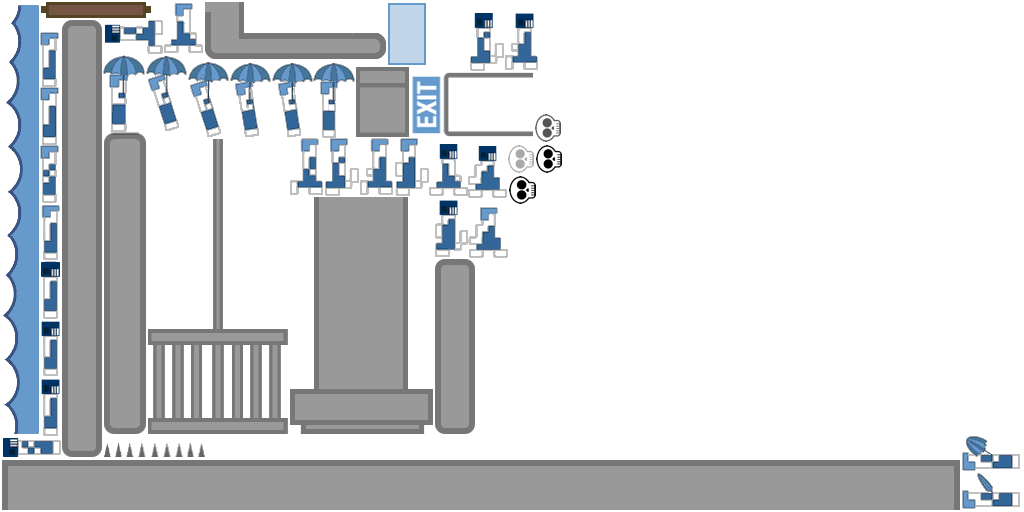
\includegraphics[width=100mm]{sources/images/Texture_atlas}
    \caption{An Example Texture Atlas}
    \label{fig:TextureAtlas}
\end{figure}

\subsubsection{Random number generation} 

Based on some very quick tests carried out by a poster on the official Cocos2D forums, I was surprised to see the difference in speed between different random number generators (RNGs) \cite{:2011zt}. It turned out that the RNG I had chosen to use (arc4Random) was by far the slowest method tested. Based on the tests carried out, I instead decided to use the CCRANDOM\_0\_1 function, which was shown to be 5 times quicker (see Figure \ref{fig:RNGTests} for the results). Although the tests carried out on the forum were tested by performing 5 million iterations of the algorithm, far more than I would ever need to use, every performance enhancement helps.
	
\begin{figure}[h!]
  \centering	
	\begin{tabular}{|l|c|c|}
		\hline
		Algorithm & Avg. Device Time (secs) & Avg. Simulator Time (secs) \\ \hline
		Ranrot & 0.037009 & 0.004949 \\ \hline
		UNI (multiply with carry) & 0.286865 & 0.015244 \\ \hline
		CCRANDOM\_0\_1 (C random) & 0.515386 &  \\ \hline
		xorrand & 1.886464 & 0.094858 \\ \hline
		arc4random & 2.858723 &  \\ \hline
	\end{tabular}    
	\caption{Performance Tests of Random Number Generators}
	\label{fig:RNGTests}
\end{figure}

\subsection{SlideViewer}

As I had a number of screens which were intended to present information to the player, I wanted to design some kind of reusable asset which could be dropped into my game and used to display this information. To this end, I created the \emph{SlideViewer class}, which as the name suggests, consists of a number of `slides' (which are simply images), which can be navigated through at the player's leisure.

The viewer is an extension of the base Sprite class, and so can be added to any other layer or sprite, and is extendable to cope with any number of slides.
		
\section{Problems Faced} 

Something which I found particularly tricky about using Objective-C over a language like Java was the memory management. Learning Objective-C really emphasised to me how much the Java runtime shields the programmer from the low-level bugs associated with memory management thanks to its garbage collector. In Java, memory is reserved for an object simply by using the 'new' keyword, and memory is automatically released when that object goes out of scope and is no longer accessible. Languages such as Objective-C  require manual memory management, meaning that every object created needs to be manually released by the programmer. While Objective-C does come with a few optimisations which make memory management easier, it still caused me a number of problems. 

I found that the biggest problem with memory leaks is that they can often go undetected, only to cause the program to unexpectedly crash later on down the line, making them very difficult to track down. I discovered a particularly nasty bug for example in my game's update method (which is called every frame), whereby I was allocating an array to hold all of the game objects, but failing to release the memory at the end of the method. This was a relatively small leak, but it was causing my game to drop 10+ frames per second if run for over 10 minutes. I found another seemingly insignificant bug in my update method which was caused by a careless error I made when initialising the game. When a level was first loaded, I wanted to create a list of all collideable objects for use in collision detection later. To do this, I put code in the update loop which added every object to a list. However, rather than just adding the objects once when the game was initialised, I found that I was re-adding each object every frame, causing a huge issue with performance. After just 10 seconds, I found that my list of collideable objects contained over 10,000 objects, which was obviously causing big problems when it came to checking for collisions. Another problem I frequently came across which couldn't happen in memory-managed languages like Java was that of uninitialised variables. Whereas in Java, whenever you declare a new variable, it's automatically initialised with whatever the default value may be, you get no such privilege in Objective-C. When you declare a variable in Objective-C, it stays uninitialised until you specifically set it. This caused me the biggest problems with arrays; trying to access an uninitialised array wouldn't cause a compiler error, but would cause an unexpected crash at runtime.

Xcode comes with a very useful set of performance analysis tools called 'Instruments' which can be used to establish any memory-related or runtime issues, such as memory leaks etc. Instruments allows you to test your app in `profiling' mode, which tracks what memory has been allocated, and suggests areas where memory leaks may occur.

\begin{figure}[h!]
  \centering
    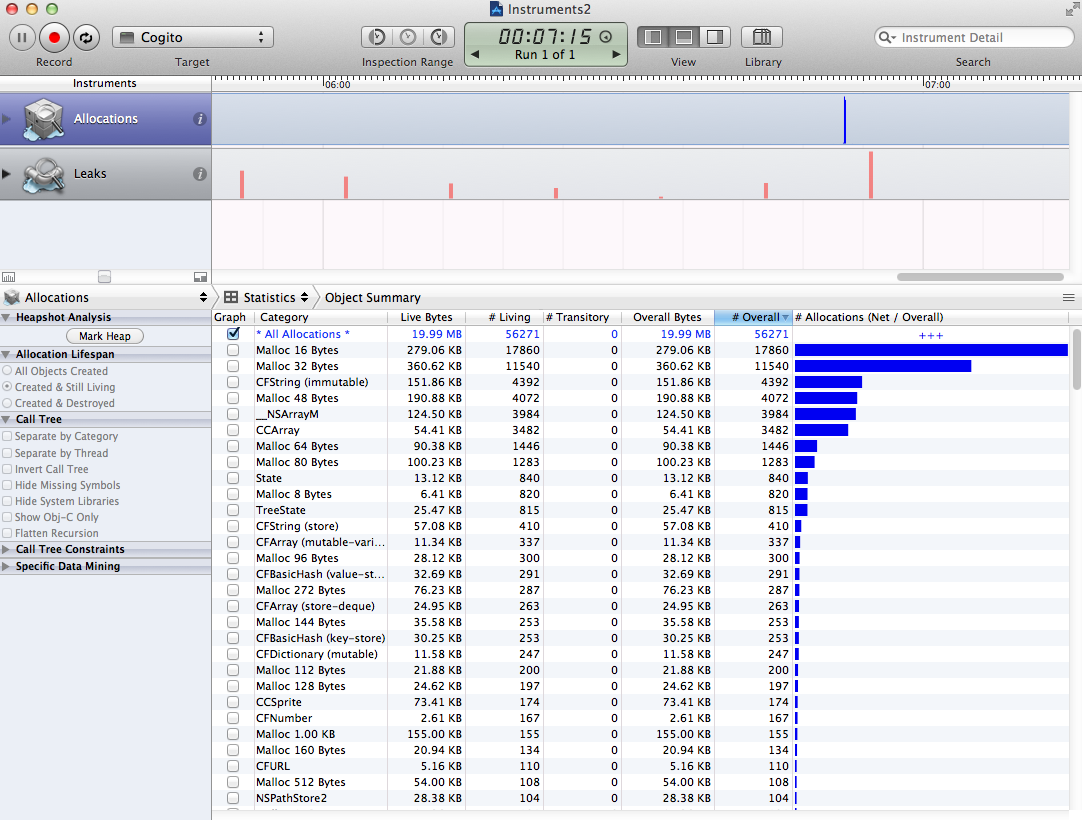
\includegraphics[width=100mm]{sources/images/Instruments}
    \caption{The Instruments Tool}
    \label{fig:TextureAtlas}
\end{figure}

Memory management aside, I had another ongoing issue with my game rating algorithm. The issue arised because I introduced a time penalty for longer games. This meant that every game to use many learning episodes was given an `F' rating, even if all agents survived. For simplicity, it would be easiest to just remove this time penalty. 

Carrying out this project really taught me the importance of keeping a close eye on what memory is being allocated and where it was being released (if at all). What may at first seem like a negligible memory leak can build up over time, and combined with other similarly small memory leaks, can cause big problems with your programs performance. I would even go so far as to say that these smaller memory leaks are even more troublesome than the bigger ones, as they are much harder to track down, and are often more widely spread, and therefore more difficult to fix.

\chapter{AI Component}

\section{Level Structure}

In order to simplify the decision making process, I split my levels into a number of `nodes' similar to the navigation meshes used in many games (See Figure \ref{fig:LevelNodes}). These nodes represent decision points in my levels; areas where there is more than one possible action to choose from, and the agent has to decide which route to take. As trapdoors had already been placed in the level, these were used as one type of decision node. I also needed to create an additional invisible decision object which could be placed at the end of platforms (or anywhere where I couldn't place a trapdoor). 

\begin{figure}[h!]
  \centering
    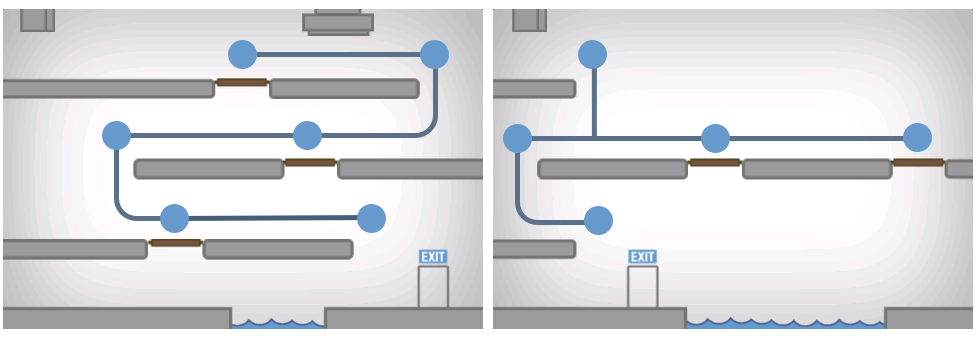
\includegraphics[width=140mm]{sources/images/LevelNodes}
    \caption{Decision Node Graphs for Two Levels}
    \label{fig:LevelNodes}
\end{figure}

\section{Learning Agents}

In my final game, I implemented three alternative methods of learning: a shortest route method, a modified decision tree method, and a reinforcement learning method using the Q-learning algorithm. As I was implementing more than one learning technique, I designed the code for my game characters in such a way that the AI was completely self-contained in its own class (see Figure \ref{fig:AgentHierarchy} for the hierarchy). Not only is this generally good object-oriented design, but it also meant that to use a different type of learning, all I had to do was to link the relevant class, no other changes were required. This functionality could be neatly implemented in a switch statement (See Listing \ref{lst:LearningType}).

\begin{figure}[H]
  \centering
    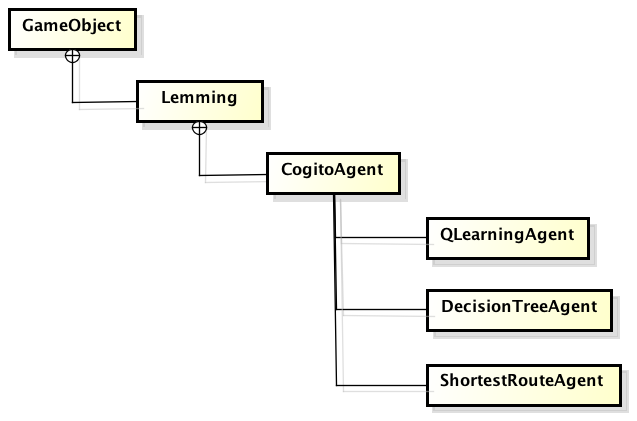
\includegraphics[width=90mm]{sources/images/GameObject}
    \caption{Learning Agent Class Hierarchy}
    \label{fig:AgentHierarchy}
\end{figure}

\begin{lstlisting}[label={lst:LearningType},caption=Switch Statement for Setting Learning Type]
switch(learningType) 
{                
	case kLearningMixed:
    	// randomly choose a learning type
        learningType = [Utils generateRandomNumberFrom:0 to:kLearningMixed]; 
        break;
                
    case kLearningReinforcement:
        class = [QLearningAgent class];
        break;
                
    case kLearningTree:
        class = [DecisionTreeAgent class];
        break;
                
    case kLearningShortestRoute:
        class = [ShortestRouteAgent class];
        break;
         
    case kLearningNone:
        class = [CogitoAgent class];
        break;
                
    default:
        break;
}
\end{lstlisting}

As outlined in my initial design, the learning agents begin the game in a `learning mode', in which they have a set number of lives or `episodes' (set by the player before the game begins). During the learning mode, the agents navigate the level and choose actions at random, building up their knowledgebase. I initially planned to set up the learning such that after the first episode, the agent would cease to act randomly and apply its knowledge. However, I found that doing this made it extremely difficult to measure the improvement in the agents, as once they reached the exit, the game was over; the learning mode avoids issue. Programming the agents to act randomly during the learning mode removes the `exploitation' element, and ensures that optimal routes are be found much quicker. Many RL systems begin to exploit learnt knowledge much earlier on, and so must balance the exploitation of existing knowledge with the exploration of new terrain. After all learning episodes have been completed, the agent then uses its knowledge to attempt to reach the exit safely.

\subsection{Cogito Agents}

I created a base class called \emph{CogitoAgent} to contain the common functionality which would be shared between all types of learning. Its main function is to detect when an agent has reached a decision node object and build an array of the available actions.

\subsection{Shortest Route Agents}

The Shortest Route agent is by far the simplest of all of the learning types. It simply records each taken route, and chooses the shortest one. I created a Route class to simplify this which consists of an array of visited `nodes' and a boolean flag which stores whether the agent survived. As the agent progresses through the level, each visited state is added to the route array. At the end of an episode, the complete route is added to a list of taken routes (see Listing \ref{lst:Shortest}). When the learning is over, the agent checks the array of taken routes, and takes the shortest one. If there happen to be several routes of the same length, the agent just picks the first one it finds, making no attempt to analyse further. If the agent failed to reach the exit at all during the learning mode, it simply acts randomly.

\begin{lstlisting}[label={lst:Shortest},caption=Updating the Route]
// add the state to the current route
[currentRoute addState:_state withAction:action];
        
if(endConditionReached) 
{
    // set the end condition
    if([_state getGameObject].gameObjectType == kObjectExit) [currentRoute setSurvived:YES];
    else if(self.state != kStateDead) [currentRoute setSurvived:NO];
            
    // add the route to routes
    [routes addObject:currentRoute];
                        
    // start new route
    currentRoute = [[Route alloc] init];
}
\end{lstlisting}


\subsection{Decision Tree Agents}

As discussed in the planning section, my decision tree implementation doesn't use classification, but instead uses a tree structure to dynamically build a model of the environment as the agents explore it. When the agent begins to explore, it sets the first state it reaches as the root node of the tree. Each succeeding state is then added to the tree in sequence (see Listing \ref{lst:TreeRoute} for a slightly simplified version of the code). If the agent has died or reached the exit, the node is set as a leaf.

\begin{lstlisting}[label={lst:TreeRoute},caption=Building a Route Tree]                       
if(levelTree == nil) levelTree = treeState; // if the root isn't set
else
{
	// add the state to the tree
    [treeState setAction:currentAction];
    [currentState addChild:treeState]; 
}
            
// update the current state/action variable
currentState = treeState;
                        
if(endConditionReached)
{
    // if we've reached an end condition, make a leaf node
    if(self.state == kStateDead) [treeState setAsLeafNode:kStateDead];
    else if([_state getGameObject].gameObjectType == kObjectExit) [treeState setAsLeafNode:kStateWin];
}        
\end{lstlisting}

At the end of the learning mode, the `route tree' is searched, with any successful routes stored. I do this using a simple depth-first search. While this kind of search is poor speed-wise, it doesn't prove an issue with the size of my levels. If I was traversing a much larger tree, I would use a heuristic search such as A* to provide an approximate solution. Upon finding a leaf node, I recursively move back up the tree building the route (see Appendix C for the code). The search of the tree continues until all nodes have been searched. After the routes have been found, I then calculate a `weight' for each route, which represents the number of tools used in that route. The final step is to find the shortest route of those found. Initially, only route lengths are checked; if there is more than one shortest route, the one with the lowest weight is chosen. This encourages the agents to choose `cheaper' routes.
  
\begin{figure}[H]
  \centering
    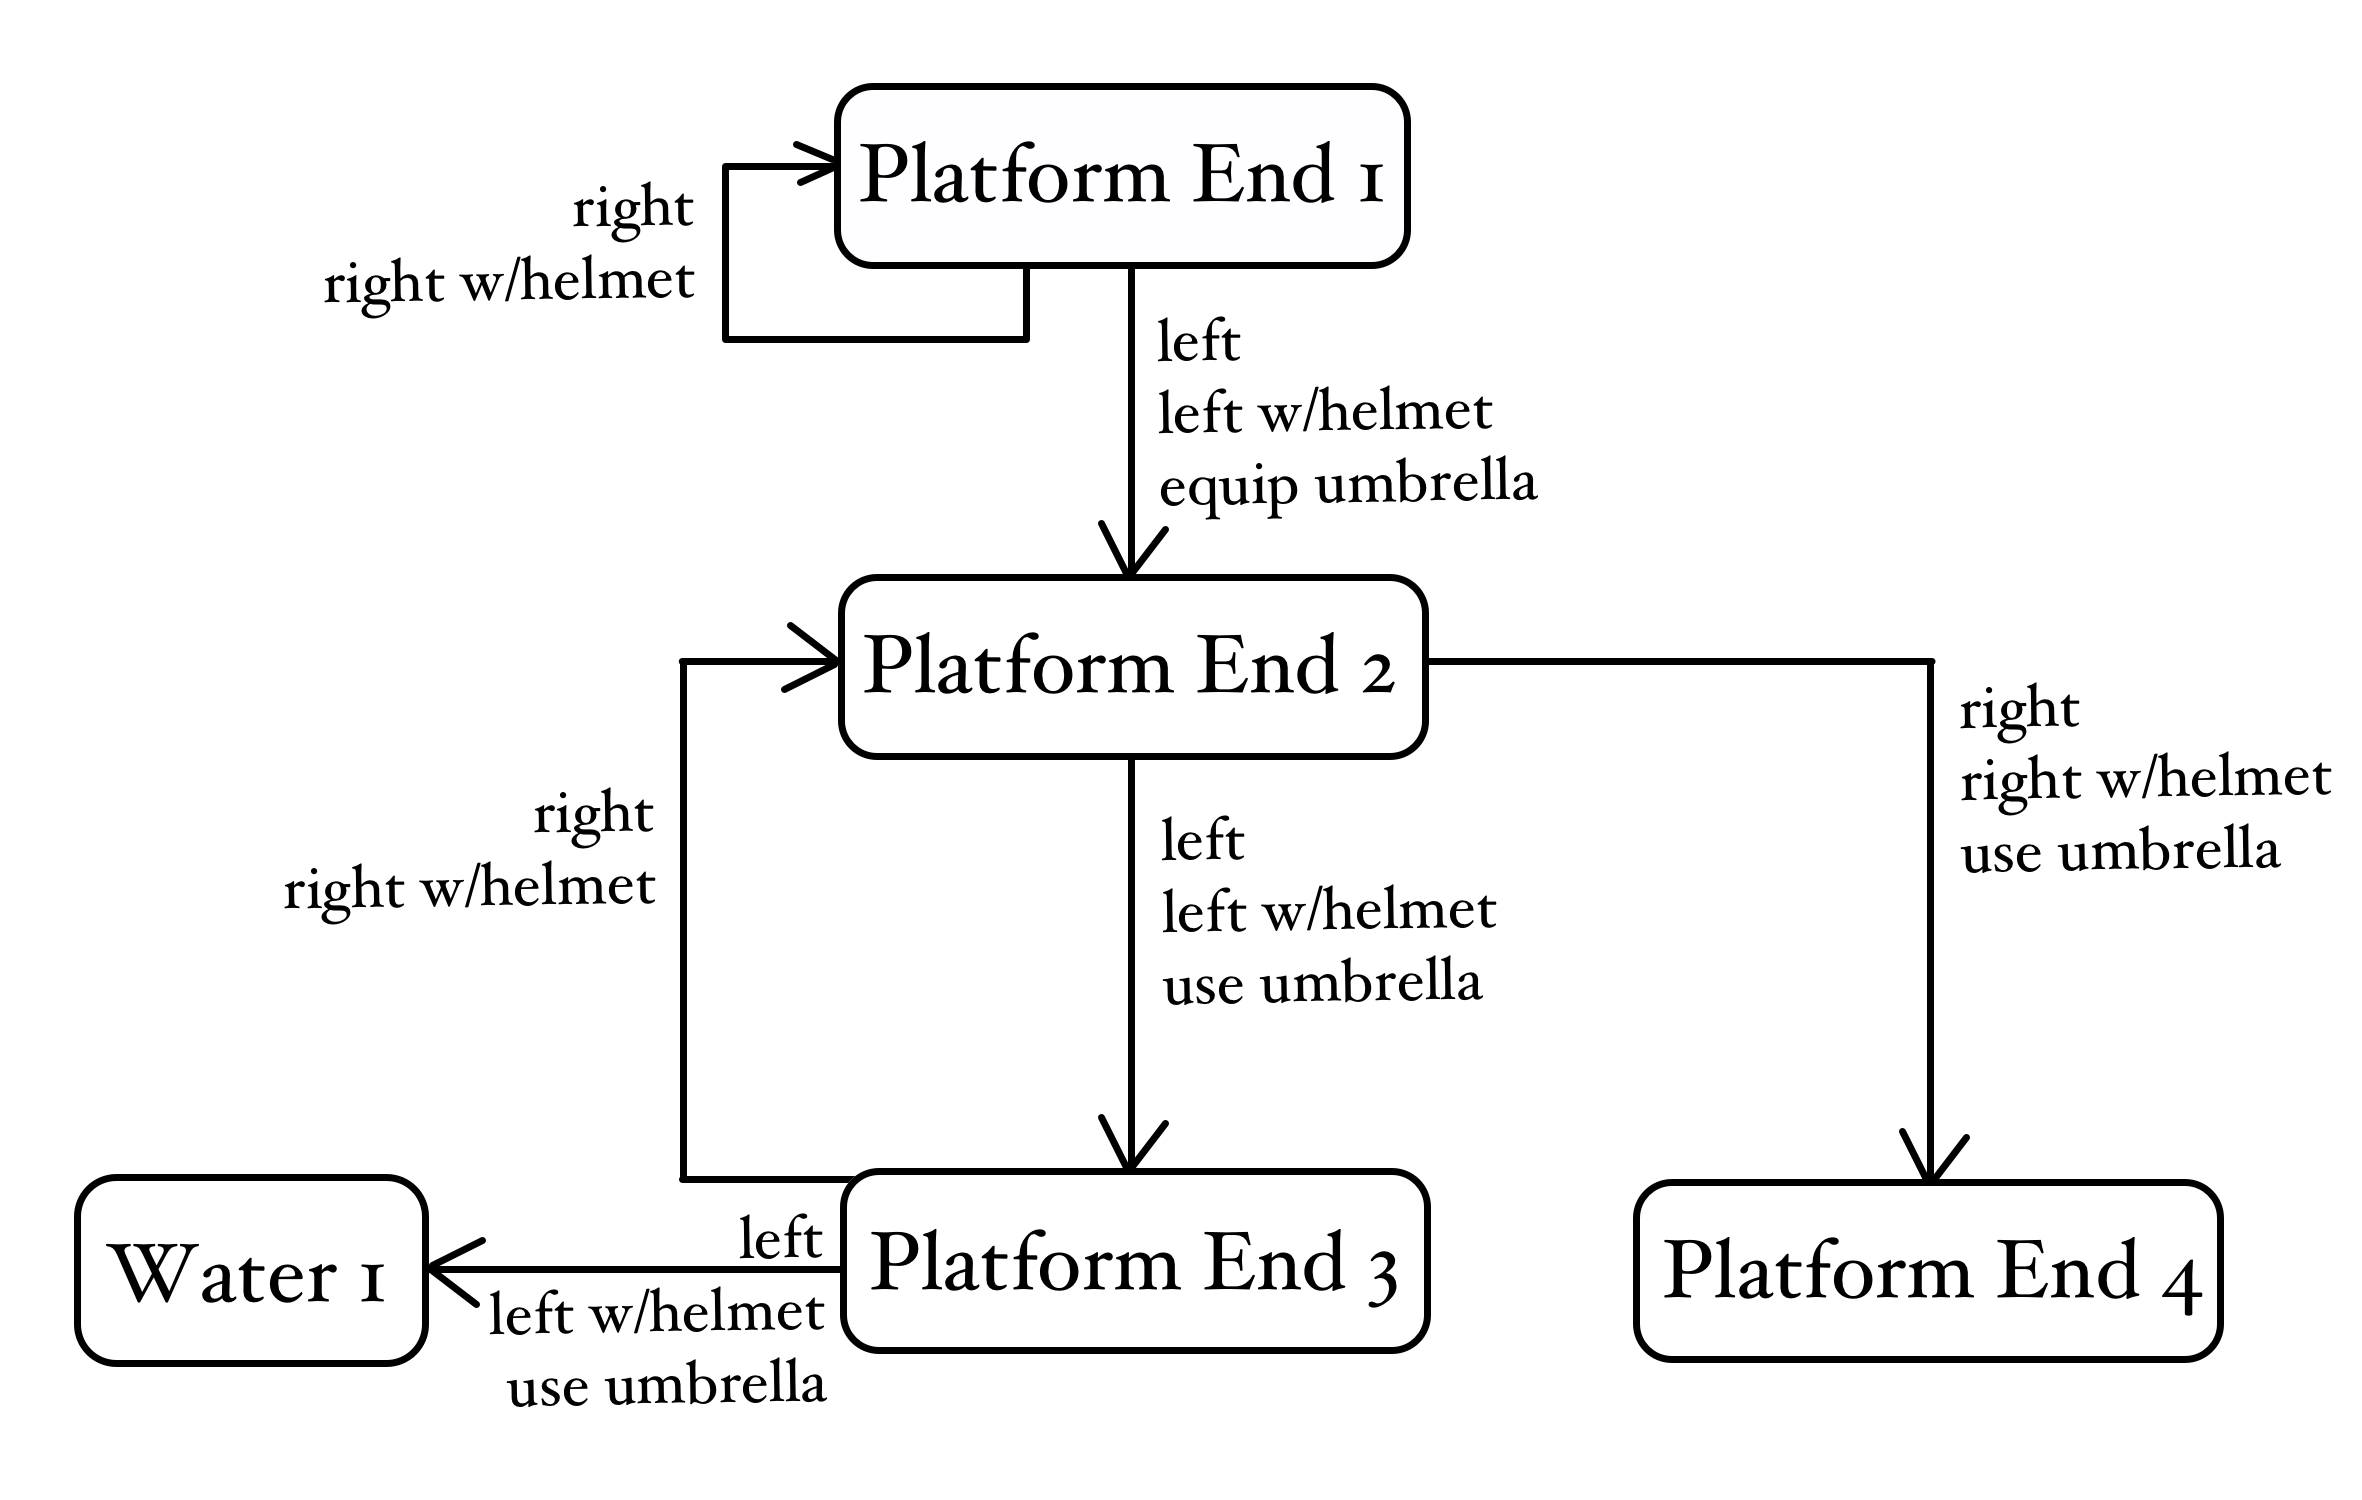
\includegraphics[width=100mm]{sources/images/TreeSample}
    \caption{A Partially-Built Level Tree}
    \label{fig:TreeSample}
\end{figure}

\subsection{Reinforcement Agents}

\begin{wrapfigure}{r}{0.42\textwidth}
\centering
\begin{tabular}{| l | c |}
  \hline
  State  & Reward Value \\
  \hline
  Reached Exit    &  100.0 \\
  Died   		  &  -100.0 \\
  Used Tool       &  -7.0 \\
  Other  		  &  -2.0 \\
  \hline
\end{tabular}
\caption{Table of Reward Values}
\label{fig:Rewards}
\end{wrapfigure}

The reinforcement agents are the most advanced of those implemented. Based on my research, I decided to use the Q-learning algorithm because I initially specified that my agents wouldn't have access to a model of the environment. The first step in implementing the algorithm was to set the reward values for my system. I used equivalent values for the win/death rewards so that both states were regarded equally `important' by my agents. In addition to these main rewards, I added a small negative reward for any tool use by the agent, to encourage less tool uses (as tools are a finite resource). As a result of my research, I also decided to give a small negative reward for every action taken by the agent, as it encourages the agents to take the shortest possible route \cite{Ng:uq}. See Figure \ref{fig:Rewards} for the values.

The agents' learning process is actually fairly simple: at the beginning of the game, the agents explore randomly. When they reach a decision node, they update the Q-value for the current state and action pair the Q-learning algorithm:

\begin{equation*}
Q(s_t,a_t) \Leftarrow Q(s_t, a_t) + (1 -\alpha_t) + \alpha[R(s_t) + \gamma max Q(s_{t+1}, a_{t+1})] 
\end{equation*}

According to the outcome of the previous action, the Q-value will either increase or decrease, with a higher value signifying a more effective action. Q-learning's use of the maximum Q-value causes a backward propagation of rewards, meaning that as more exploration takes place, the rewards `diffuse' to the other states, essentially leaving a trail to the goal. The agents continue to navigate the level and update the Q-values until they have completed all learning episodes. Unlike my other learning methods, there is no need to calculate and store the optimum route beforehand. All that is needed is for the agent to begin traversing the level as usual. Upon reaching a decision node, the agent simply checks the Q-values of the actions available, and chooses the action with the highest Q-value (see Listing \ref{lst:OptimumQ} for the code). This process is repeated until the agent (hopefully) reaches the exit. 

\begin{lstlisting}[label={lst:OptimumQ},caption=Finding the Optimum Action For the Current State]                       
Action optimumAction = -1;
float maxQValue = -1000000;
CCArray* actions = [self getActions];
    
for (int i = 0; i < [actions count]; i++) 
{
    float qValue = [self getQValueForAction:[[actions objectAtIndex:i] intValue]];
    if(qValue > maxQValue) 
    {
        maxQValue = qValue;
        optimumAction = [[actions objectAtIndex:i] intValue];
    }
}
return optimumAction;
\end{lstlisting}

My implementation of the algorithm is slightly different to that described in Watkins' paper \cite{Watkins:1989mi}. In the paper, when an agent moves to a new state, the Q-values for \emph{that} state are updated. As my agents have no prior knowledge of their environment, this would be impossible. To circumvent this, the agent instead updates the Q-values for the previous state. Although this is slightly different to the standard method, it has no impact on the actual learning.

To make my code more readable, I split the algorithm into logical parts and stored these parts in variables. I created a variable for the old Q-value (i.e. $Q(s_t, a_t)$), a variable for the maximum expected Q-value (i.e. $max Q(s_{t+1}, a_{t+1})$) and a variable for the reward (i.e $R(s_t)$). I chose to update the Q-values asynchronously (i.e. updating individual Q-values at each decision made), rather that to update all Q-values at set intervals because I felt it was more logical and also slightly simpler to implement this way. My implementation of the Q-Learning update algorithm can be seen in Listing \ref{lst:QLearning} (I have omitted a large switch statement for the sake of readability). Although it was contrary to my research I chose to use a high (and static) learning rate as it meant that the Q-values altered by a large amount at each update, thus increasing the likelihood of an optimal policy being found. Were my agents able to perform thousands of iterations, I would have chosen different values, but I felt this was inappropriate for my chosen application area, in which a single game is very unlikely to last for an hour, much less several hours.

\begin{lstlisting}[label={lst:QLearning},caption=Implementation of The Q-Learning Algorithm]
-(void)updateQValues:(QState*)_newState
{    
    if(currentState == nil) return;
            
    float oldQValue = [currentState getQValueForAction:currentAction];
    float maximumQValue = [_newState calculateMaxQValue];
    float reward = [_newState getReward];
    
    // apply a negative reward if using a tool
    ...
    SWITCH STATEMENT OMITTED 
    ...
        
    float updatedQValue = oldQValue * (1 - kQLearningRate) + kQLearningRate 
    	* (reward + kQDiscountFactor * maximumQValue);
    [currentState setQValue:updatedQValue forAction:currentAction];
}
\end{lstlisting}

In addition to a more powerful algorithm, my reinforcement agents are also able to utilise a central knowledgebase. This meant that the rate of learning could be greatly increased, with 100 agents performing just one learning episode each being the equivalent to a single agent performing 100 episodes. I also added the ability to export the knowledgebase to an external file saved in the iOS device's memory for later analysis.

\section{Learning Stats}

I added an additional game stats screen to the game's main menu which gives the player a simple summary of the performance of the agents. I do this using a number of visual bar graphs, which are updated dynamically using the data collected after every completed game. I display these stats using my \emph{SlideViewer} object.

\section{Problems Faced}
	
Fortunately, I didn't encounter any major issues when it came to implementing my learning. One fairly minor problem that I did come across was that I found it was possible for agents to get stuck in an `infinite decision loop'. After an agent had finished learning, it was possible for it to transition to a state whereby there was only one possible decision point (see Figure \ref{fig:InfiniteDecisionLoop} for an example). If actions in this state led to death, an agent could keep moving back and forth, making it impossible to complete the game.

\begin{wrapfigure}{l}{0.52\textwidth}
  \centering
    
\includegraphics[width=70mm]{sources/images/Screen_InfiniteLoop}
    \caption{An Example of a Possible `Infinite Decision Loop' State}
    \label{fig:InfiniteDecisionLoop}
\end{wrapfigure}

The problem was being caused because I had programmed my agents to stop learning once the learning mode was over. My solution to this problem therefore was to allow the agents to continue to update the knowledgebase after the learning mode was complete. This worked because of the fact that I had applied a small negative reward to every action taken by the agent, meaning that were an agent caught in an infinite decision loop, the small negative rewards would build up and eventually filter to the previous states, meaning that agents would not fall into the same trap.
	
	
	
%
% New part
%

\part{Testing \& Evaluation}{This section presents the usability and learning testing I performed, the results that were obtained, and an analysis of the product's performance.}

\chapter{Testing \& Results}

In this section I present the results to my usability tests, in addition to the results from the AI testing. I initially planned to create some unit tests to test the functionality of my game. However, as the user-input was very limited, I didn't feel that this was necessary.

\section{Usability Testing and Error Checking}

As a result of my iterative development approach, the testing of my game was carried out as and when I implemented new features, fixing any bugs as they arose. As I was working alone, this was the most appropriate method. For this reason, I didn't make as much use of bug tracking software as I would if I was working in a development team. Although I did make some use of Github's built in issue-tracking to record major errors, or errors I couldn't fix at the time of their discovery.

My game was largely designed as a test for machine learning in a game environment and as such, user interaction was always intended to be limited. Due to this, the usability tests which could be carried out were similarly limited; there was little other than basic user-interface testing needed (there was no need for unit testing).

One bug that was picked up during the usability tests that I wasn't able to solve was a problem with the game pausing. I found that when resuming the game, it was possible for agents to fall though the environment. This occurred if the game was paused while the agents were mid-way through transitioning to a lower level. I think the problem was with `delay' method I used when agents use an umbrella or drop to a lower level, the problem being that the delay was cut short if the game was paused. I came up with a partial solution to this problem, although the issue does still occur if there are many agents in the level. My solution was to change how I was pausing the game. To begin with, I was manually iterating through all of the objects in the game, and pausing them one by one. To try and fix the problem, I instead decided to use a function in Cocos2D's \emph{Director} class (the same method used by the engine when the user sends the app to the background by pressing the home button).

\section{AI Testing}

In addition to the usability tests, I also carried out extensive tests of my AI system. The primary aim of these tests being to check the effectiveness of the learning techniques (i.e the level of improvement they offered), as well as to compare each technique against the others.

I first provide a summary and brief analysis of my results, which are proceeded by a series of graphs showing the results to my AI testing.

In addition to testing the learning agents, I also tested my agents without any learning. This acted as a point of comparison to measure the improvement in my learning agents. As the non-learning agents actions were completely random, it is not a surprise that their success rate was approximately 50\% (it was actually 57\%). I also recorded the average number of actions, and the average length of each learning episode for comparison purposes. As the reinforcement agents have the added option of a shared knowledgebase, I wanted to see how this affected the learning. Figure \ref{fig:SA_RL} shows how the number of agents correlates with the success rate of the agents. The results in this graph are even more impressive due to the fact that the agents only used one learning episode.

I was particularly impressed with the reinforcement learning agents, which showed the biggest improvement of all techniques. Looking at Figure \ref{fig:AvgSuccess}, we see that the reinforcement agents showed a 99\% success rate compared with just 57\% without learning. The reinforcement agents also showed a great improvement in the actual length of the routes, with the optimum routes averaging 2-3 actions, and 26 seconds. Compared with the non-learning average of 4 actions and 55 seconds, this is a considerable improvement.

The decision tree agents also showed improvement over the basic agents, with an average agent success rate of 85\%. The optimum routes were also an improvement, albeit less of an improvement when compared with the reinforcement agents. The decision tree agents' optimum routes showed an improvement of 8 seconds. In Figure \ref{fig:SE_Tree}, we see a definite correlation to suggest a greater success rate the more learning episodes are used.

I most surprised with the results for my shortest route agents. While they were by far the simplest and most naive method of those implemented, they still showed an impressive improvement over the basic agents, and even showed to be more effective than the decision tree agents (although I think this second point may be a coincidence, and would like to conduct a more in-depth analysis). The shortest route agents showed an impressive 88\% success rate. The optimum routes they chose also showed improvement over the basic agents, with an average length of 41 seconds, and using 4 actions. The shortest route agents also showed a definite correlation between the success rate of the agents and the number of learning episodes they used.

Overall, I feel that my results were very encouraging. All learning techniques which I implemented have shown a considerable improvement in all areas over the agents without any learning. All methods show an improvement in not only the percentage of agents successfully reaching the exit, but also the optimum routes found by all agents are shorter (in both time and number of actions required). My reinforcement agents proved by far the most effective technique, with a success rate of almost 100\%. I was slightly disappointed to see that my tree agents didn't really offer any improvement over the shortest route agents, despite their use of route `weighting' and the tree structure itself. I would have expected to see at least some improvement over the shortest route agents.
\newpage

\begin{figure}[H]
  \centering
    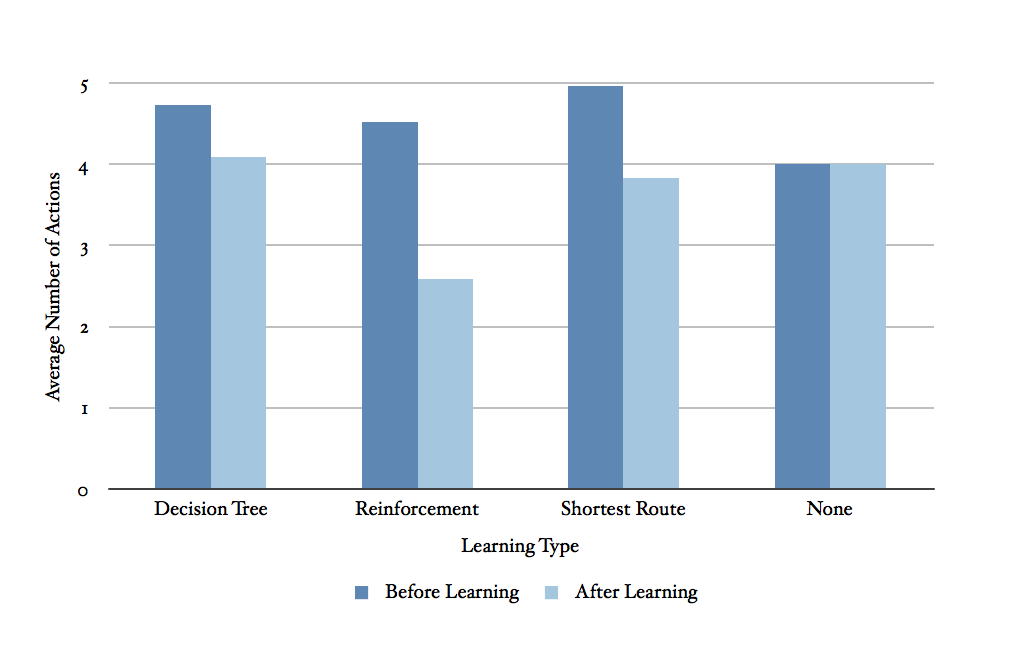
\includegraphics[width=140mm]{sources/images/AvgActions}
    \caption{Average Actions Taken Per Episode}
    \label{fig:AvgActions}
\end{figure}

\begin{figure}[H]
  \centering
    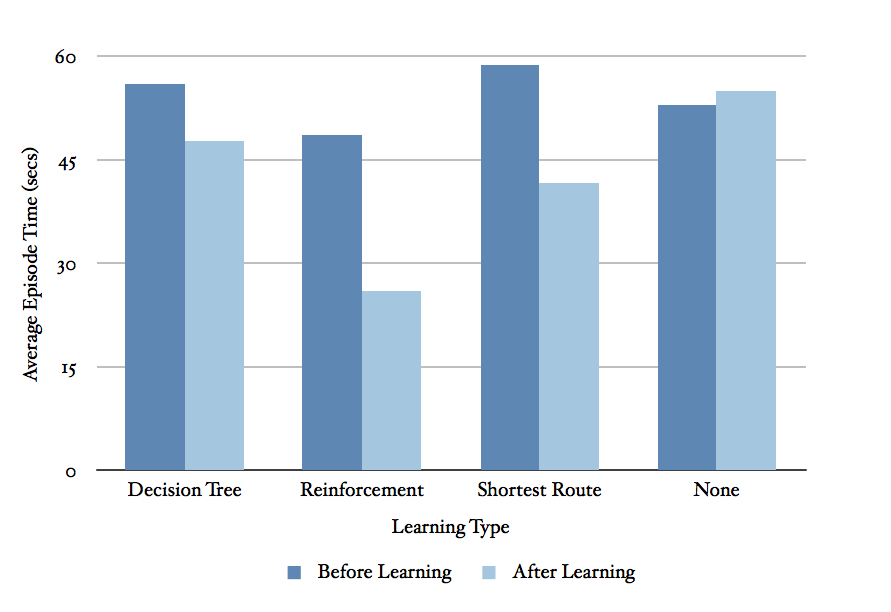
\includegraphics[width=140mm]{sources/images/AvgEpisode}
    \caption{Average Episode Time}
    \label{fig:AvgTime}
\end{figure}

\begin{figure}[H]
  \centering
    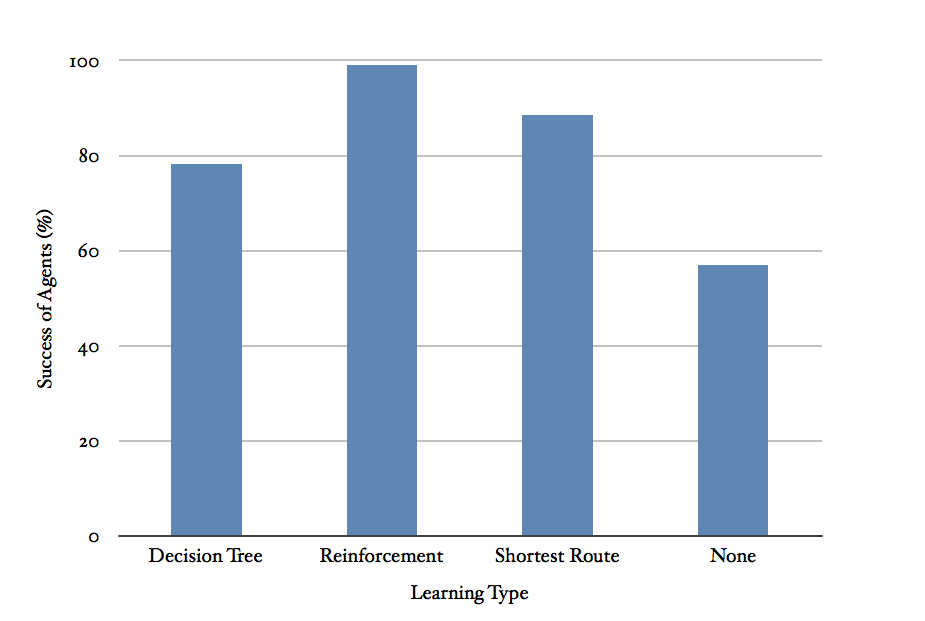
\includegraphics[width=140mm]{sources/images/AvgSuccess}
    \caption{Average Success Rate of Agents}
    \label{fig:AvgSuccess}
\end{figure}

\begin{figure}[H]
  \centering
    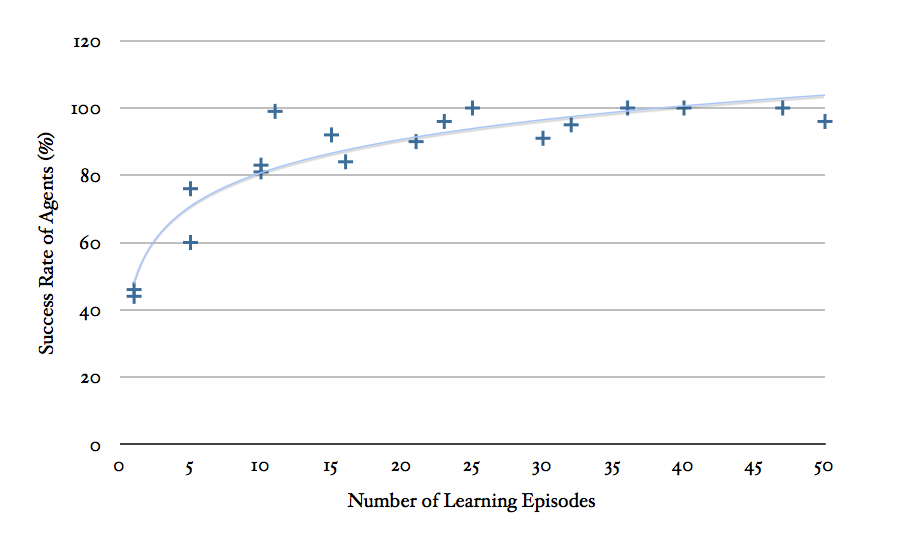
\includegraphics[width=140mm]{sources/images/SE_Tree}
    \caption{Comparing Success Rate and Number of Episodes (Decision Tree)}
    \label{fig:SE_Tree}
\end{figure}

\begin{figure}[H]
  \centering
    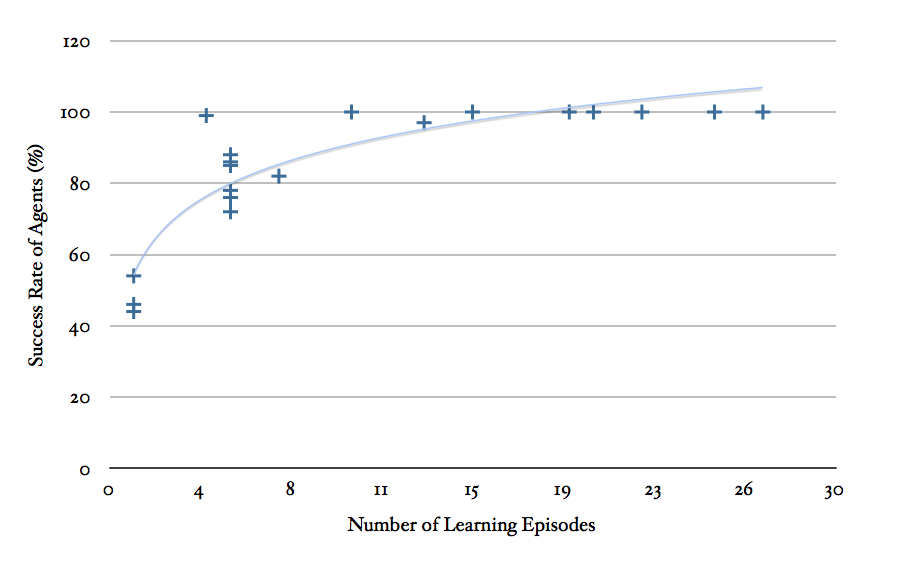
\includegraphics[width=140mm]{sources/images/SE_SR}
    \caption{Comparing Success Rate and Number of Episodes (Shortest Route)}
    \label{fig:SE_SR}
\end{figure}

\begin{figure}[H]
  \centering
    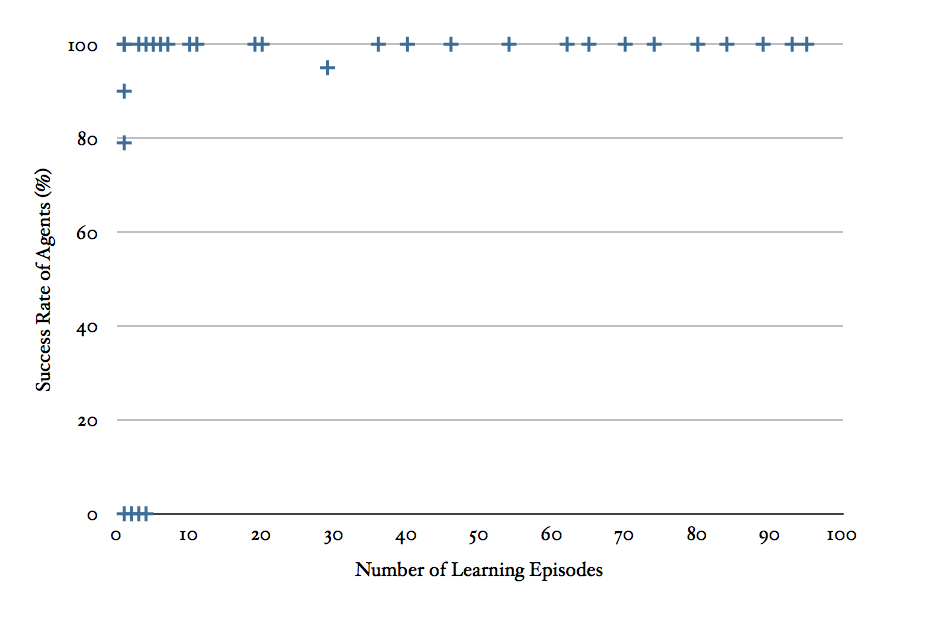
\includegraphics[width=140mm]{sources/images/SE_RL}
    \caption{Comparing Success Rate and Number of Episodes (Reinforcement)}
    \label{fig:SE_RL}
\end{figure}

\begin{figure}[H]
  \centering
    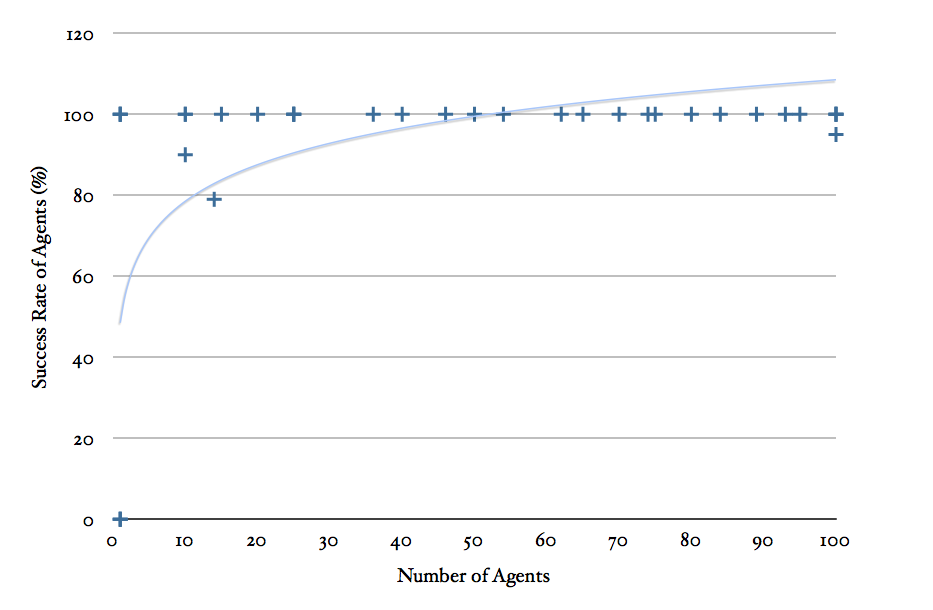
\includegraphics[width=140mm]{sources/images/SA_RL}
    \caption{Comparing Success Rate and Number of Agents (Reinforcement)}
    \label{fig:SA_RL}
\end{figure}

\newpage

\subsection{Q-Learning Policies}

As mentioned in the implementation section, I added the functionality to export the Q-values for a game. Below is an example of one such policy. I have also included a screenshot of the level in question with each obstacle labelled according to the table for further clarity.

\begin{figure}[H]
\centering    
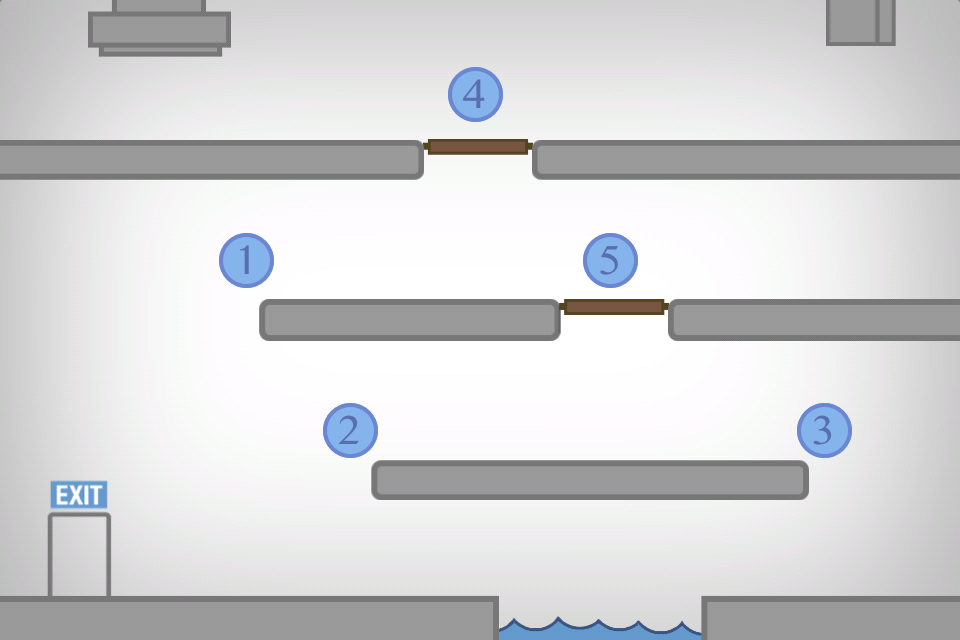
\includegraphics[width=85mm]{sources/images/Level2} \paragraph{}
    
\begin{tabular}{|l|l|c|}
\hline
Object & Actions & Q-value \\ \hline

\multirow{5}{*}{1. Terrain End (122,186)} & Equip Umbrella & 100 \\
 & Left & -1.314 \\
 & Left (helmet) & -7 \\
 & Right & 77.199 \\ 
 & Right (helmet) & 72.199 \\ \hline
 
\multirow{3}{*}{2. Terrain End (177,107)} & Equip Umbrella & 100 \\
 & Left & 100 \\
 & Right & 77.199 \\ \hline
 
\multirow{5}{*}{3. Terrain End (412,107)} & Equip Umbrella & -100 \\
 & Left & 88 \\
 & Left (helmet) & 83 \\
 & Right & -100 \\
 & Right (helmet) & -100 \\ \hline

\multirow{6}{*}{4. Trapdoor (239,240)} & Down & 87.395 \\
 & Down (umbrella) & 81.427 \\
 & Left & -100 \\
 & Left (helmet) & 70.742 \\
 & Right & 75.892 \\
 & Right (helmet) & 70.657 \\ \hline

\multirow{6}{*}{5. Trapdoor (307,160)} & Down & 81.917 \\
 & Down (umbrella) & 73.949 \\
 & Left & 88 \\
 & Left (helmet) & 83 \\
 & Right & 77.199 \\
 & Right (helmet) & 72.199 \\ \hline
 
\end{tabular}

\caption{An optimal policy for Level 2 (with 100 agents \& 19 learning episodes)}
\end{figure}

As can be seen from the table, the policy shows that the agents were able to learn which actions were best suited for which states. An example being state 4: the agents learnt that moving left would lead to death by stamper, and so has a large negative reward.



%
% New part
%

\chapter{Evaluation}

In this section, I provide analysis of my learning techniques and their effectiveness, as well as a more general evaluation of my project as a whole.

\section{Time Management}

When planning the development of my project, I intended to take a linear `waterfall' development approach, developing the game and AI components separately and testing at the end of development. I actually ended up taking a more incremental approach: developing individual features and testing as I went along. This change in approach was partly due to the fact that I was unfamiliar with the development of software in Objective-C. In terms of sticking to my initial schedule, I feel that the development ran fairly smoothly, albeit with a few slight changes to my initial plan. The biggest change being that I didn't carry out the testing phase at the end. Additionally, the actual development itself wasn't quite as modular as planned. The biggest miscalculation with my project schedule was that I failed to recognise just how much groundwork was needed to build the game component. Though I by no means expected the game development to be a trivial task, I wasn't prepared for the amount of work that was needed. This was exacerbated by the fact that I was also still getting to grips with Objective-C, and so my productivity wasn't as it could have been. However, although I slipped by a couple of weeks during the game development stage, I finished the AI component of the game under-schedule. Looking back at the volume of code that was needed to get the game running, it seems fairly obvious now that I should have at least allocated an equal amount of time to both the game and AI components. As it happens, I still finished my project to schedule with some time to spare.

\section{Analysis of Machine Learning}

Overall, the learning element of my system proved very effective. All learning types implemented showed an improvement over the agents with no learning. In this section, I provide some more in-depth analysis of each technique.

\subsection{Shortest Route Learning}

Despite being most naive method, the shortest route still provided a great improvement over the agents without learning. Advantages to this method are that it is simple to implement, is quick and computationally cheap to function and it clearly yields effective results. 

However, this method also has some significant disadvantages. The biggest being the accuracy or indeed the optimality of the `optimal' routes it produces. The obvious flaw in this method is that the `optimum' route is completely dependent on the agent actually \emph{taking} the shortest route themselves. Although this does not present a major problem with my levels, the greater the level size, the smaller the probability that the agent will discover the optimum route (or even any route at all). My results show this, although using a much greater number of learning episodes helps to avoid this. This is a problem which is only likely to increase with the size of the level. Another big disadvantage to this method is that unsuccessful routes do not contribute to the knowledgebase, so are essentially wasted time. 

There are a number of ways to improve this method. One enhancement which would greatly reduce the space complexity of the method is to remove the need to store each individual route. Instead, a single route could be stored, with a simple check at the end of each episode to determine whether the new route improved over the stored one. This would also remove the need to iterate through a long list of routes at the end of learning. Another possible enhancement is to implement a shared knowledgebase, which could take the form of a shared list of all routes, or as mentioned, be a shared copy of the optimum route so far. The benefit to using a shared knowledgebase has been proven in my Q-learning implementation; it greatly improves the efficiency and most importantly the speed of learning. Another area for improvement is in the comparison of different routes. In it's current state, the optimum route is the one which has the smallest number of moves (or actions). If multiple optimum routes exist, the first one is used. This could be greatly improved by using a weighting system similar to the decision tree method, whereby each route is given a `weight' (determined by the number of tool uses in that route), encouraging the selection of routes with less tool uses. A final improvement could be to implement some way to build a `Frankenstein' route using the pieces of the stored routes. This way, a truly optimum route could be found, even if the agent hadn't actually taken it.

\subsection{Decision Tree Learning}

Although I originally planned to implement decision tree learning, I didn't feel that my problem could be solved using classification, and so my tree method takes a slightly different approach. Unlike most decision tree learning methods, my implementation dynamically creates a map of the environment in a tree structure as the agent progresses. It takes a similar approach to the shortest route method but improves upon the storage space required by only storing states once. A big advantage to this method over the shortest route is that even unsuccessful episodes contribute to the knowledgebase to be used later. It also improves over the shortest route's route selection process by calculating `weightings' for the routes, which encourages the choice of routes with less tool uses. As with the shortest route method, it provides a considerable improvement over the agents with no learning. It also offers an improvement to the length of the optimum route when compared with the shortest route. 

However, my decision tree method also shares some of the pitfalls of the shortest route method. One such problem being the fact that it is similarly reliant on the agents discovering an optimal route whilst they are exploring the environment. As with shortest route, the chance of even completing the level successfully decreases as the level size grows, so relying solely on this is not preferable. This method is also more computationally expensive and slower than the shortest route method, as the tree must be exhaustively searched and an `optimum' route built. As it is, I don't feel that this method provides a great enough improvement over the shortest route method to justify the extra computation needed.

One improvement which could be made could be to provide some more powerful route `filtering' to determine optimal routes. A simple way to do this is to incorporate the route's length into its weighting (currently the algorithm only uses the weightings to compare two routes of the same length). This would produce `cheaper' routes than at present, as it would prefer routes which may be slightly longer, but don't use as many tools. Another improvement could be to introduce a shared knowledgebase, greatly increasing the chance of finding an optimal route. Finally, a more efficient search method could be used in anticipation of using much larger levels. An heuristic algorithm such as A* would be appropriate.

\subsection{Reinforcement Learning}

Overall, my RL agents performed even better than expected, with the agents able to fairly quickly gather enough information to formulate an optimum policy. In addition, after a reasonable amount of episodes, the method gave a 100\% survival rate which is as good as can be expected. Another big advantage to this method is that every decision made by the agents contributes to the knowledgebase in a positive way; an agent dying is as helpful as an agent reaching the exit, if not more so, as it teaches the agent where \emph{not} to go. The algorithm is also capable of functioning in much larger environments (given enough storage space). It also requires very little computation to build the optimum policy after the learning is complete, as the agent only needs to search through the actions currently available to it for the current state. There is no need to search through vast knowledgebases, or build a route beforehand. For this reason, I feel that this method is particularly suited to a game environment, where high performance is paramount.

However, there are also a few problems with this method. One being the amount of storage space required. The algorithm requires that a Q-value is stored for every action/state combination tried by the agent. While this is not an issue in my game due to the small environments, this could be problematic in much larger environments - especially if using mobile hardware. Another problem with my implementation in particular is that it never truly converges, so the route taken by the agent is not necessarily the optimum route. The main cause for this is the limited amount of time given to learn; as the method relies on a backwards propagation of rewards, it can take some time for said rewards to transfer to the farthest corners of the level. Many machine learning systems are run for several thousand iterations, giving enough time for convergence. With each episode in my game taking 1-2 minutes, it isn't feasible for my AI system to run for this many iterations. My addition of a shared knowledgebase greatly helped with this, using many agents to simultaneously contribute to the same knowledgebase, greatly reducing the time required for an optimal solution to be found. 

Although my RL agents proved to be very effective, there are a few improvements which I would make given more time. One such improvement being the addition of a variable learning rate. I discovered from my research that many RL systems begin the learning with a high learning rate, reducing it as time goes on, which makes learning quicker early on, with more fine-tuning to the system later, resulting in more accurate policies. I made the decision during the implementation stage to use a fixed rate as it would produce results much faster, which is key in a game environment; players don't have time to wait for hours for the AI to adjust. Another small enhancement I would make is to provide some way to save and load policies. Doing this and updating the same policies would allow the policies to converge, resulting in much more accuracy. The final enhancement that I'd like to make would be to implement some additional RL algorithms such as bucket brigade.

\section{General Areas For Enhancement}

Although I'm very pleased with the outcome of my project, given extra development time, there are a number of areas which I feel I would like to extend further.

The first and perhaps most obvious enhancement that I would make would be to extend my system to use more learning types. I would like to experiment with genetic algorithms in particular, as I think that they lend themselves quite well to the context of my game. Each individual agent could represent a chromosome, with only those agents with the shortest/cheapest routes being chosen for `breeding'. The agents could spawn in waves, with the algorithm being performed after each wave to represent a single generation. This functionality could be built on top of the existing shortest route method, which stores each route in an array. The breeding/mutation process could be performed by splicing the two parent agents's routes.

Another enhancement that I think it would be interesting to make would be to allow for multiple learning types to be used in a single game, with separate agents able to use different algorithms. It would be interesting to compare the performance of the methods in real-time. 

I would also like to implement some way for the agents to learn from each other - perhaps by `watching' (or being in the vicinity of) other agents. This wouldn't be as effective as using a shared knowledegebase, but it would create some more diverse behaviour among the agents, rather than every agent using the same route. While not necessarily appropriate to my problem area, it could definitely be useful in commercial games, where the AI agents need to appear realistic by employing a diverse range of behaviour.

I would also like to introduce much bigger levels into my game with more diverse obstacles. Although the agents show a definite improvement in their traversal of the levels, I don't feel that such small levels allow my system to fully demonstrate its capabilities. I did initially look into creating levels which were several screen-widths wide, with the player able to scroll along the level. However due to the size restrictions of the iPhone screen, I later decided against this as I felt it was bad from a usability point of view, as the majority of the game level would be obscured from the player. It would perhaps be more appropriate to create a version of the game for a desktop computer with much bigger levels.

A small criticism I have of my system is that it is very specific to the individual levels; the information learnt about one level is completely useless for another (a problem known as overfitting). Overfitting is a known `flaw' of the Q-learning algorithm. In an ideal scenario, an agent would be able to generalise its experiences to apply the learnt knowledge in different scenarios, however, this would be virtually impossible in my case. A possible solution to overfitting could be to develop the AI in two components: one using Q-learning to learn the policy for that individual level, and another (possibly a genetic algorithm) to learn more general rules. 

\section{The Project in Context}
	
I feel that the modules studied throughout my course set me up well for carrying out this project, and there are many skills I have learnt along the way which I took advantage of when developing my product.

There was obviously a lot of knowledge that I gained in the AI-related modules I have studied (CI213 - Intelligent Systems and CI342 - Advanced AI) which I could directly apply to my project. Techniques such as pathfinding algorithms, and generally approaching AI-based problems from an academic angle.

I was also able to apply a lot of useful knowledge that I had gained from the programming-based modules from my course (CI101 - Introduction to Programming, CI228 - Object-Oriented Software Design and Specification and CI346 - Programming, Concurrency and Client-Server Computing). I applied a lot of the `good' object-oriented design practices which were learnt in these modules: principles such as inheritance and design patterns like the singleton. I also found the knowledge learnt this year in CI346 very useful to overcome some concurrency issues I had using multiple threads in my system.

Another module I have found to be very useful is CI224 (Games Development). Many of the game design concepts: physics, object transformations, model loading, and various other useful skills. The project we did in CI224 was particularly useful, as it introduced me to the processes involved in developing a game from scratch. I was also introduced to source control systems in CI224, which has proven to be invaluable knowledge to have.

I also used the knowledge of object-oriented software design and UML learnt in CI228 and CI231 (Formal Underpinnings and Specification) to design my system. Although I didn't actually use the formal specification language learnt in my system specification, I could still apply the concepts learnt to my own designs.

I learnt a great deal about data access and performance optimisation in the CI312 (Computer Graphics Algorithms) module. It really helped me too look at my code at a lower level, and analyse the best and most efficient ways to access and manipulate data; something which I have found to be incredibly important, especially in a game context, where some functions can be called 60 times every second.

\section{Conclusion}

I feel that overall, my project was a great success; I achieved my initial goal of creating AI agents capable of learning how to traverse my game levels. Although some methods proved more effective than others, all of the techniques I implemented showed a marked improvement over the basic (non-learning) agents. I was particularly pleased with the reinforcement agents, which have proven very effective in finding the optimum solution in a relatively limited number of learning episodes. Particularly so when utilising the shared knowledgebase. 

Learning aside, I was also very pleased with the core `game' component; especially given the fact that I had to create the artwork and character animations, and program the core game myself. I feel that the final game is very robust, and serves well to demonstrate my AI system especially given the initial problems I encountered due to my inexperience in using Objective-C.

I feel I have learnt a great deal carrying out this project. Aside from the knowledge of AI and machine learning, I have also learnt a considerable amount about more general software and game development. Having never developed a software product from concept to completion, carrying out the initial design, specification development and testing was invaluable and gave me an insight into the development process. I found this project to be particularly useful from a game development point of view, due to the fact that I was developing for mobile hardware. Because of this, there were a number of considerations which I had to make such as the reuse of assets and using optimised file formats; issues which are often forgotten because of the powerful hardware at our disposal today.

In conclusion, I feel that I suitably demonstrated that it is not only possible, but computationally feasible with today's technology to implement machine learning techniques in games. This is made even more pertinent considering that I did so on a mobile device (although I accept that not many games have the same amount of processor time to devote to the AI as my project). Such techniques could have many possible applications in games to create much more `intelligent' AI systems capable of dynamically modifying their behaviour to adapt to the player. Given that machine learning techniques have been shown to be effective in commercial games (Lionhead's Black \& White being the flagship example), it is surprising to me that more developers haven't taken up the mantle and implemented similar techniques in their own games. Such techniques could be applied to virtually any game genre, from enemy commanders in a real-time strategy war game, to the AI-controlled players in a football game. Given the increase in priority of the AI (more processor time, and dedicated AI programmers), such techniques are likely to become more widespread in the near future. 



%
% References
%

\singlespace

\newpage
\addcontentsline{toc}{part}{Bibliography}
\bibliographystyle{abbrv}
\bibliography{Cogito}



%
% New part 
%

\part{Appendices}{}
\appendix
\onehalfspace

\section{Appendix A: Project Schedule}
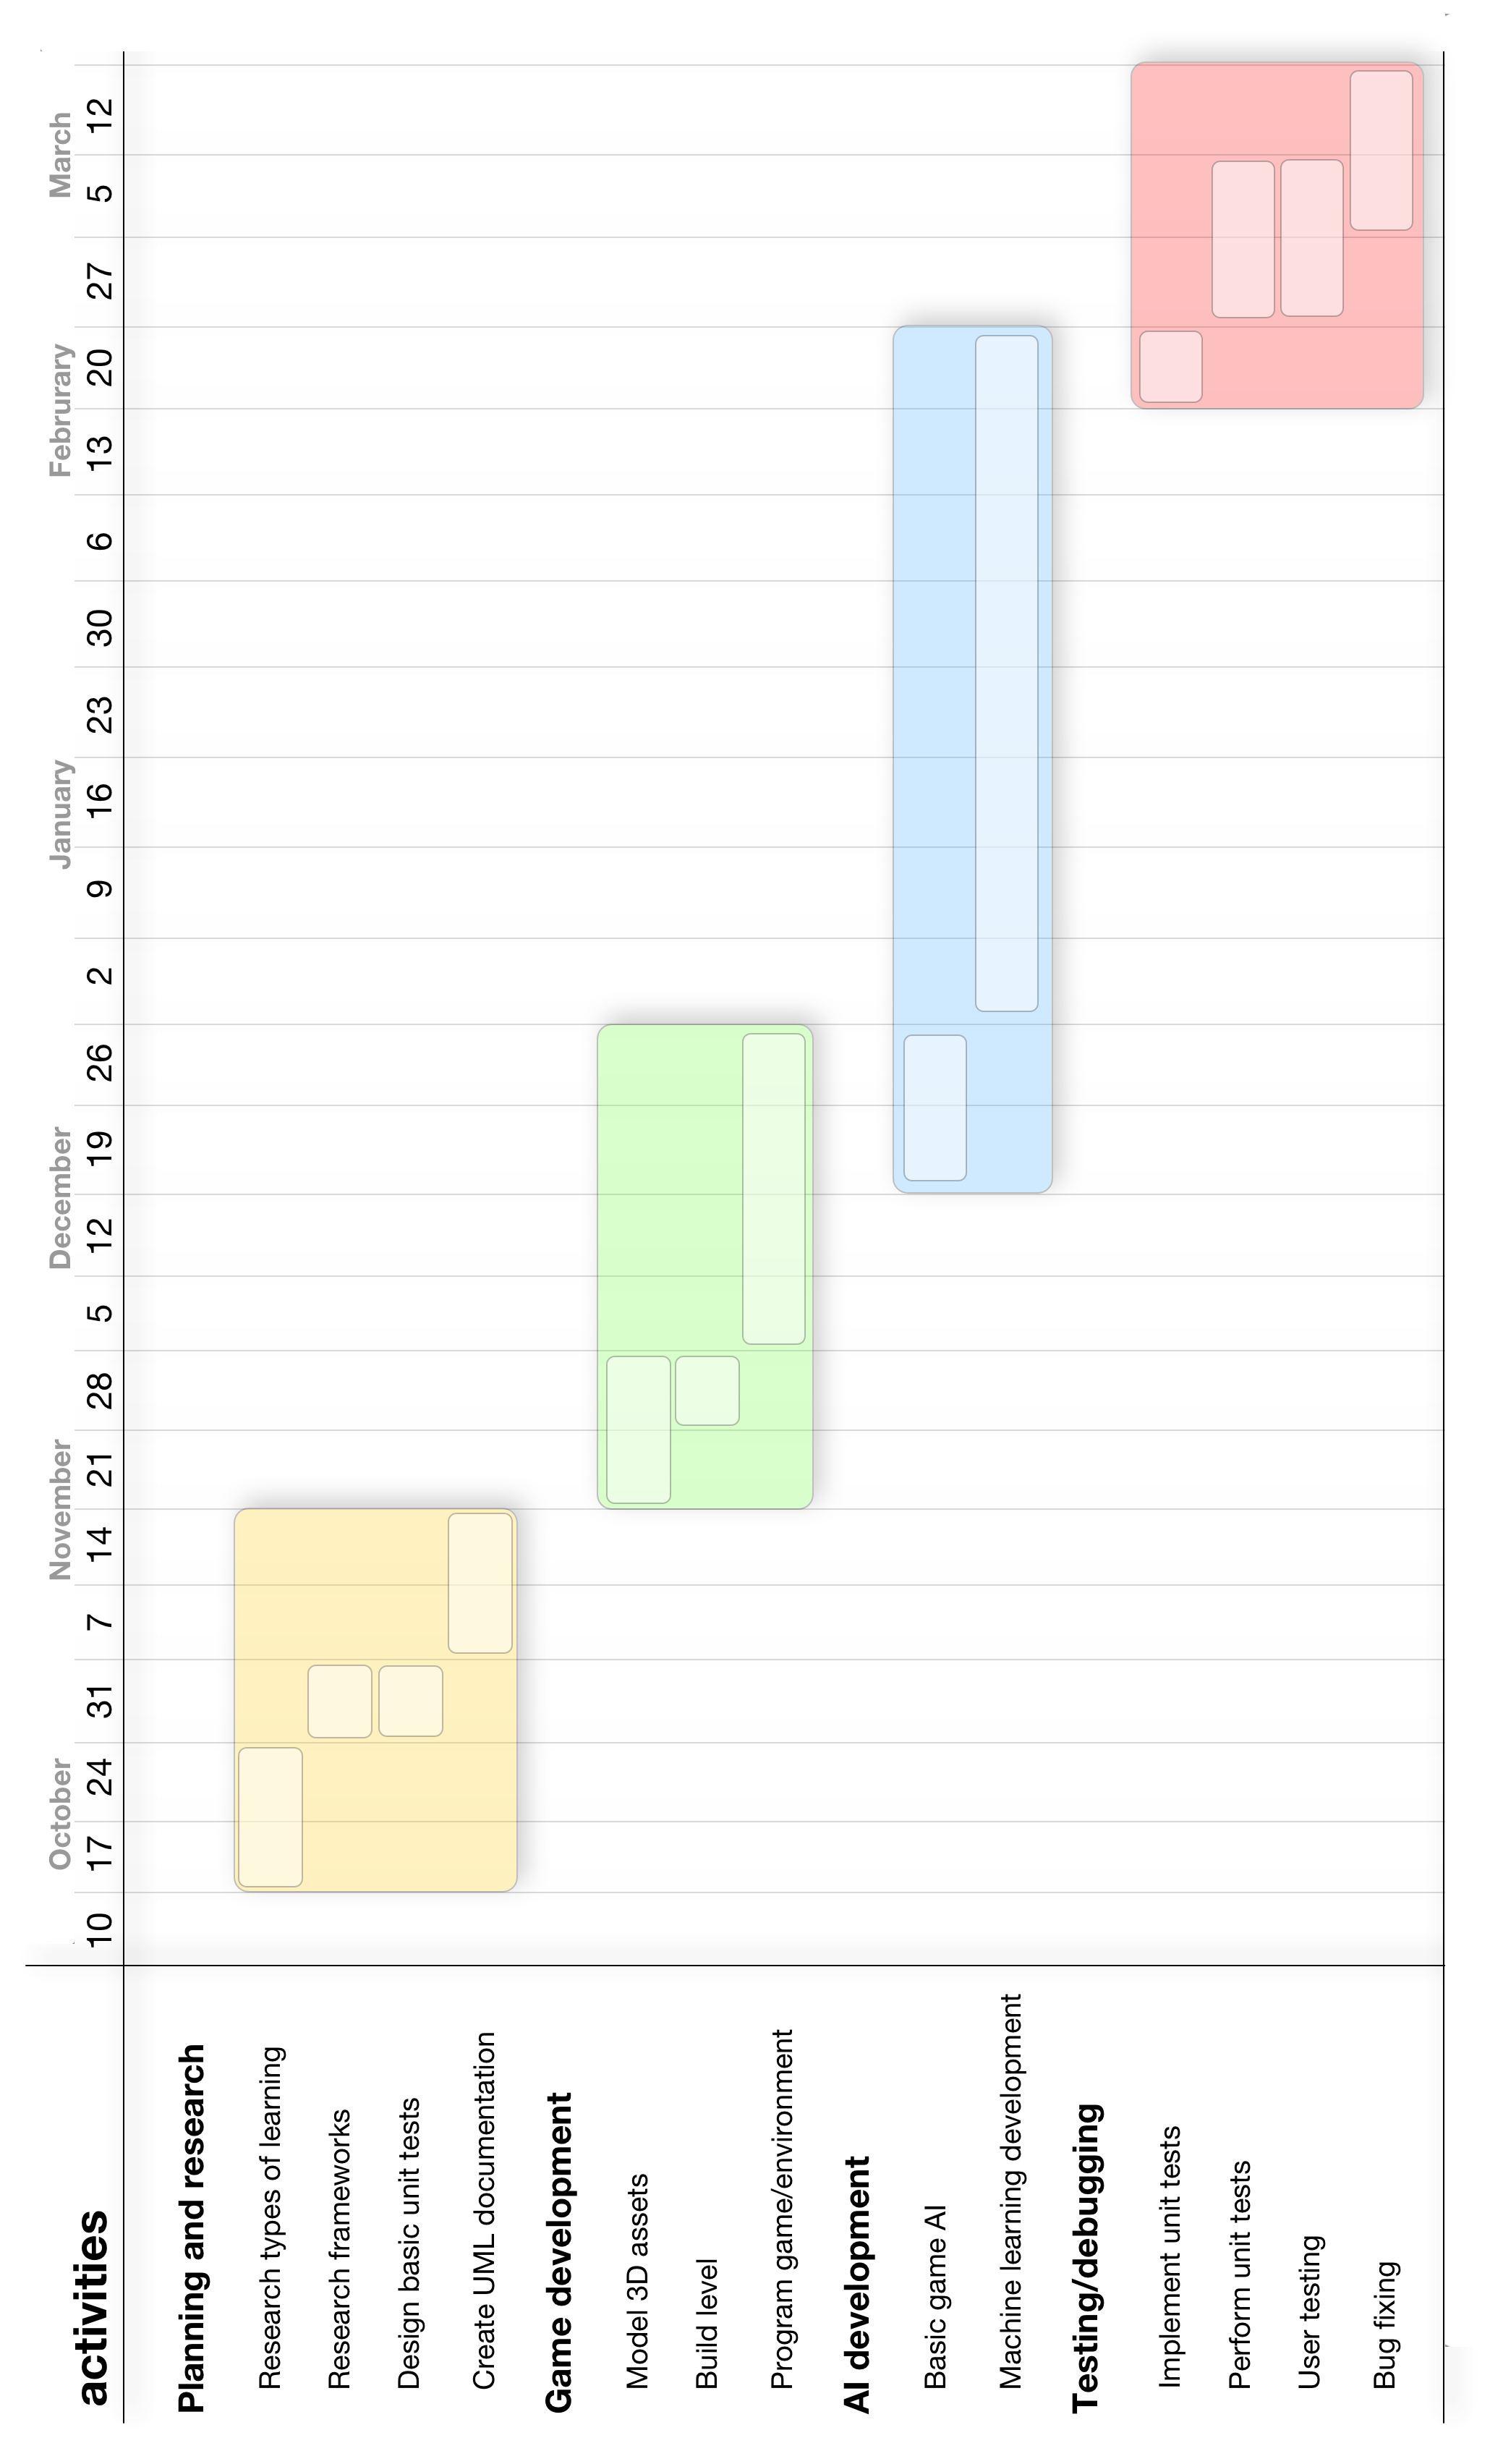
\includegraphics[width=140mm]{sources/images/Schedule}

\section{Appendix B: Collision Detection}
\begin{lstlisting}
-(void)checkForCollisions:(CCArray*)_listOfGameObjects
{
    CCArray* collisions = [CCArray arrayWithCapacity:0];
    CGRect selfBBox = [self adjustedBoundingBox];
    BOOL colliding = NO;
    
    for (GameObject *gameObject in _listOfGameObjects) 
    {
        // no need to check for self-self collisions
        if(gameObject == self || gameObject.gameObjectType == kLemmingType) continue;
        
        CGRect objectBBox = [gameObject adjustedBoundingBox];
        if(CGRectIntersectsRect(selfBBox, objectBBox)) 
        {
            [collisions addObject:gameObject];
            if(gameObject.gameObjectType == kObjectTerrain || gameObject.gameObjectType == kObjectTrapdoor) colliding = YES;
        }
    }
    
    // check if the lemming should be falling
    if(!colliding && state != kStateSpawning && state != kStateFalling && state != kStateFloating && state != kStateDead) [self changeState:kStateFalling];
    
    // work out what we're actually colliding with, and call onObjectCollision
    if([collisions count] > 0)
    {
        if([collisions count] > 1) // if we're colliding with two objects
        {        
            GameObject* object1 = [collisions objectAtIndex:0];
            GameObject* object2 = [collisions objectAtIndex:1];
            
            if(object1.gameObjectType == kObjectTerrain || object2.gameObjectType == kObjectTerrain) 
            {
                if(object1.gameObjectType == kObjectTerrain) object = object2;
                else object = object1;
            }
        }
        else object = [collisions objectAtIndex:0];
        
        if(![object isCollideable]) return;

        if(object.gameObjectType == objectLastCollidedWith) 
            if(object.gameObjectType != kObjectTerrain && (self.state != kStateFalling || self.state != kStateFloating)) return;
        else objectLastCollidedWith = object.gameObjectType; 
        [self onObjectCollision:object];
    }
}
\end{lstlisting}
\newpage

\section{Appendix C: An Example Level Specification}
\begin{lstlisting}
<dict>
	<key>Entrance</key>
	<dict>
		<key>type</key>
		<string>terrain</string>
		<key>isCollideable</key>
		<false/>
		<key>x</key>
		<integer>240</integer>
		<key>y</key>
		<integer>310</integer>
		<key>filename</key>
		<string>entrance</string>
		<key>objectType</key>
		<string>entrance</string>
	</dict>
	<key>Level2_Platform1</key>
	<dict>
		<key>type</key>
		<string>terrain</string>
		<key>x</key>
		<integer>71</integer>
		<key>y</key>
		<integer>160</integer>
		<key>filename</key>
		<string>platform_medium</string>
	</dict>
	<key>FloorPiece1</key>
	<dict>
		<key>type</key>
		<string>terrain</string>
		<key>x</key>
		<integer>-60</integer>
		<key>y</key>
		<integer>10</integer>
		<key>filename</key>
		<string>floor</string>
	</dict>
	<key>Exit</key>
	<dict>
		<key>type</key>
		<string>terrain</string>
		<key>objectType</key>
		<string>exit</string>
		<key>x</key>
		<integer>40</integer>
		<key>y</key>
		<integer>50</integer>
		<key>filename</key>
		<string>exit</string>
	</dict>
</dict>
\end{lstlisting}
\newpage

\section{Appendix D: Optimum Route Calculation (Tree)}
\begin{lstlisting}
-(void)setOptimumRoute
{    
    // build the routes
    CCArray\* routes = [self getShortestRoutes];
    
    // if no optimum routes are found, exit
    if([routes count] == 0) return;
    
    // calculate the cost of each route (cost = +1 for every tool use)
    NSMutableDictionary\* routesWithCosts = [NSMutableDictionary dictionaryWithCapacity:[routes count]];
    
    for (int i = 0; i < [routes count]; i++) 
    {
        CCArray\* route = [routes objectAtIndex:i];
        int routeCost = 0;
        
        for (int i = 0; i < [route count]; i++) 
            if([[route objectAtIndex:i] getAction] == kActionDownUmbrella ||
               [[route objectAtIndex:i] getAction] == kActionEquipUmbrella ||
               [[route objectAtIndex:i] getAction] == kActionLeftHelmet ||
               [[route objectAtIndex:i] getAction] == kActionRightHelmet) 
                    routeCost++;
        
        [routesWithCosts setObject:[NSNumber numberWithInt:routeCost] forKey:route];
    }
    
    // find the route with the lowest cost
    int minimumCost = 999;      // the lowest cost so far
    CCArray\* minimumCostRoute;
    
    for (CCArray* route in routesWithCosts) 
    {
        if([[routesWithCosts objectForKey:route] intValue] < minimumCost)
        {
            minimumCostRoute = route;
            minimumCost = [[routesWithCosts objectForKey:route] intValue];
        }
    }
    
    // finally, the array needs to be reversed
    for (int i = [minimumCostRoute count]-1; i > -1; i--) 
        [optimumRoute addObject:[minimumCostRoute objectAtIndex:i]];
}
\end{lstlisting}
\newpage

\section{Appendix E: Resources Disk}

\textbf{[the resources disk can be found inside the back cover of this report]} \\

The attached resources disk contains a variety of useful resources, including the full source code, graphical assets and generated HTML documentation. There are three folders in the root level of the disk: 

\subsection{documentation} The documentation folder contains the documentation generated using \emph{Doxygen}. The documentation is in HTML format, and can be run from the index.html file located at: \url{/documentation/html/index.html}. This HTML documentation lists every class used in my program, and gives a summary of every method and variable used. The documentation folder also includes PDF copies of the Process Report and the Project Log.

\subsection{media} The media folder contains some additional multimedia assets. I have included a short video which highlights the functionality of my system, which can be found here: \url{/media/CogitoTrailer.mov} (I have also included MP4 and WMV versions of the video). I have also included some sample data collected from my program in the form of the raw plist files, which can be found in: \url{/media/GameData}. The main \emph{GameData.plist} file contains a list of the played games and relevant stats. There are also 10 example policies output by my reinforcement learning system. 

\subsection{src} The src folder contains all of the source code for my project, the content graphics, the level data and the Cocos2D framework code. I have also included the Xcode project file in this folder for reference.

\subsection{System Requirements}

My system requires a Macintosh system to build and run. The system can be tested using the iOS Simulator program included with Apple's Xcode IDE or an iOS device.

\begin{itemize}
	\item Intel-based Mac running Mac OS Snow Leopard or later
	\item Xcode 4 or later installed
	\item To test on iOS devices, an iPhone 3GS or later running iOS 4+ is required (must also be registered in the Apple Developer Program to test on iOS devices).
\end{itemize}

\end{document}
